% REMEMBER: You must not plagiarise anything in your report. Be extremely careful.
\documentclass{l4proj}

%==================================================================================================
% Put any additional packages here
% You can add any packages you want, as long as it does not alter the overall format (e.g. don't change the margins or the reference style).
%
\usepackage{pdfpages} % if you want to include a PDF for an ethics checklist, for example
\usepackage{enumitem}
\usepackage{hyperref}
\usepackage{float}
\usepackage{physics, amsmath, amssymb, graphicx, fancyvrb}
\usepackage{multirow}


\begin{document}

%==================================================================================================
%% METADATA
\title{Automatic Illustration of Text via Multimodal Interaction}
\author{Stergious Aji (2546916A)}
\date{\today}

\maketitle

%==================================================================================================
%% ABSTRACT
\begin{abstract}
    (TODO)

    This paper describes a system that automatically illustrates textual information present in audio sources, in addition to a ground truth construction interface for automatic videography generation systems.
    
    Users can use this system as a standard automated videography tool that generates videos with relevant imagery appearing in time with the text in the audio. Alternatively, they can build ground truth data for various audio sources. This ground truth would consist of timing information as well as sets of true labelled images for each chunk within the audio.

    
    
    % Every abstract follows a similar pattern. Motivate; set aims; describe work; explain results.
    % \vskip 0.5em
    % ``XYZ is bad. This project investigated ABC to determine if it was better. 
    % ABC used XXX and YYY to implement ZZZ. This is particularly interesting as XXX and YYY have
    % never been used together. It was found that  
    % ABC was 20\% better than XYZ, though it caused rabies in half of subjects.''
\end{abstract}

%==================================================================================================
%% ACKNOWLEDGEMENTS
% \chapter*{Acknowledgements}
% Enter any acknowledgements here. This is optional; you may leave this blank if you wish, or remove the entire chapter
%
% We give thanks to the Gods of LaTeX, who in their eternal graciousness, have granted that this document may compile without errors or overfull hboxes.

%==================================================================================================
% EDUCATION REUSE CONSENT FORM
% If you consent to your project being shown to future students for educational purposes then insert your name and the date below to  sign the education use form that appears in the front of the document. You must explicitly give consent if you wish to do so.
% If you sign, your project may be included in the Hall of Fame if it scores particularly highly.
%
% Please note that you are under no obligation to sign this declaration, but doing so would help future students.

\def\consentname {Stergious Aji} % your full name
\def\consentdate {\today} % the date you agree
\educationalconsent


%==================================================================================================
\tableofcontents
%==================================================================================================
%% Notes on formatting
%==================================================================================================
% The first page, abstract and table of contents are numbered using Roman numerals and are not included in the page count. 
%
% From now on pages are numbered using Arabic numerals. Therefore, immediately after the first call to \chapter we need the call \pagenumbering{arabic} and this should be called once only in the document. 
%
%
% The first Chapter should then be on page 1. 

% PAGE LIMITS
% You are allowed 40 pages for a 40 credit project and 30 pages for a 20 credit report. This includes everything numbered in Arabic numerals (excluding front matter) up to but *excluding the appendices and bibliography*.
%
% FORMATTING
% You must not alter text size (it is currently 10pt) or alter margins or spacing. Do not alter the bibliography style. 
%
%==================================================================================================
%
% IMPORTANT
% The chapter headings and structure here are **suggestions**. You don't have to follow this model if it doesn't fit your project. Every project should have an introduction and conclusion, however.  If in doubt, your supervisor can give you specific guidance; their view takes precedence over the structure suggested here.
%
%==================================================================================================
\chapter{Introduction}
% reset page numbering. Don't remove this!
\pagenumbering{arabic} 

% Why should the reader care about what are you doing and what are you actually doing?
This chapter serves to outline the motivations for creating an automatic videography tool, as well as the rationale for a subsequent interface for annotating ground truths, specifically using multimodal representations of images and text. 

% \textbf{Motivate} first, then state the general problem clearly. 
\section{Motivations}
\subsection{Automatic Videography of Audio}
Text-to-image retrieval is a topic that has gained increased interest in recent years due to the advent of new deep-learning approaches that has considerably outperformed prior work. Following this, these advancements have illuminated new innovation into areas like automatic content creation. The rise in video production \citep{tprisevideo} has demanded a drive for more automated systems, especially in the realm of music. On popular platforms like \cite{youtube}, music often lacks accompanying video content which can be due to various reasons such as a lack of funding and resources or song popularity. More commonly, many older music tracks that previously only existed in analogue formats have been digitised to be uploaded to the platform.

Moreover, this tool has applications beyond music tracks, as it can effectively enhance educational materials and podcasts. Incorporating multiple modes of information, such as visual, audio, and textual, can increase the accessibility of the subject and improve user engagement and retention. According to the study by \citep{benefits_of_mmv} participants who watched a video lecture with both visual and auditory content outperformed those who watched a lecture with only one of those elements. As a result, incorporating video into educational materials could provide a better learning experience that caters to the diverse learning styles identified in Fleming's VARK acronym \citep{vark}.

One of the main motivations of this project is to build on and enhance previous work on the Automatic Videography of Audio Tracks of Songs by \cite{parker}. Parker's thesis achieved a functioning video generation tool, focused on audio tracks sourced from YouTube, however, it suffered from a number of drawbacks that we aim to resolve with this project. A more in-depth review of the thesis is conducted in Section \ref{sec:background_parker} of the Background.

\subsection{Ground-Truth Annotation Interface}
With an evergrowing supply of automatic videography systems, it is important to perform evaluations and compare their relative performances. Nevertheless, we have found that there is a lack of objective procedures for evaluating comparative performances between different videography systems. More specifically in measuring their accuracy at image retrieval from text. Image relevance can and has been assessed with qualitative user surveys but this can often be very subjective and sensitive to personal preferences and present moods. More importantly, to evaluate a new system, further user studies must be conducted with the same demographic of people if the goal is to compare against the results of a previously evaluated system. This is impractical, not to mention, time-consuming, ultimately producing unrepeatable and biased results.

This can be mitigated if instead, a set of true labels are annotated beforehand for provided audio sources which can then be used to evaluate any number of videography systems on those same audio sources. It is vital that a static image collection is used for ground truth constructing and evaluating in order to produce repeatable and standardised performance metrics.

This called for a user-friendly interface to assess the relevance of images from the textual content present in the inputted audio source. Under the hood, this ground-truth constructor interface can use the same pipeline as the automated videography system that we are creating. 


\section{Aims}
This project aims to produce a piece of software that can take any audio source and automatically generate a video from it. The video will consist of timely imagery corresponding to the textual content present in the audio. In addition, this software will include a novel annotation interface for assessing image relevance from text prompts. This will let the user construct a set of ground truths for each portion of the given audio source. This will be achieved by letting the annotator select the set of images that they perceive as the most fitting to the accompanying text or song lyric in the given chunk of audio. This set of images will be picked from a top-$k$ which will be retrieved using our system.

Since there is a high priority for precise ground truth construction, the software must be intuitive to use with clear instructions for the user to follow. We must, therefore, aim to produce a user-friendly interface in an easily accessible platform. Additionally, since the aim is for anyone to use this application, appropriate error handling must be in place to accommodate users from a wide range of technical backgrounds. We also aim to make our system modular in design. This way, more technical users would be able to swap in any image collection with minimal configuring if required.

We aim to provide a set of completed ground truths for a pre-defined list of audio sources using our annotation interface. This data will be made available in an accessible format so that it can be used to measure the quality of existing and future videography systems using standard Information Retrieval (IR) metrics like Average Precision, F-Measure, and Normalised Discounted Cumulative Gain (nDCG).

Finally, as stated in our motivations, we wish to fix the limitations of the previous videography generation system by Parker as well as expand upon its functionality. We aim to, generalise the application of the tool to any audio source, not just restrict it to sourcing from YouTube videos. This also means, our tool must be able to support the transcription of multiple languages. We aim to tackle the image retrieval process using a different approach that introduces semantics in order to retrieve more relevant images.

% However, the data will not be restricted to the task of automatic videography, due to it simply consisting of a set of relevance assessments of images from text. Hence, the data can be used in existing or new text-to-image research in general. A recent example of such a possible use case is investigating the effeciveness of Variable Depth Pooling (CITE), more details are discussed in the Background section \ref{sec:background_pooling}.

% In order to justify creating a novel annotation interface, we must first explore existing solutions and their corresponding strengths and limitations.


%==================================================================================================
\chapter{Background}
This chapter serves to lay the foundations in order to contextualise this project within the field of Information Retrieval (IR). Firstly, a look into the origins of the field, specifically text-to-image retrieval, will be conducted. This will be followed by a discussion of the recent advancements in computer vision to allow multimodal representations of images with natural language. We will briefly look into the history of relevance assessment to ground our problem of evaluating IR systems and justify our proposed approach. Next, the previous thesis on automatic videography will be critiqued, with the aim of identifying its merits and shortcomings. This will form the basis for which our project will build upon. Finally, an outline of what current solutions exist to solve our problem of assessing the relevance of images from text queries will be provided.

\section{The History of Image Retrieval}
Image retrieval is an important branch within the field of IR which has evolved over the past several decades. Recent years have witnessed an exponentially growing collection of images, spanning various domains such as academia, medicine, social media, and the military. This makes it all the more imperative that efficient mechanisms are in place to scour these databases. The earliest such mechanisms can be traced back to the 1970s. Known plainly as Text-Based Image Retrieval (TBIR) systems, they relied on keyword-based querying of a relational database \citep{chang1979tbir}. Consequently, every image in the database had to be labelled with appropriate keywords and a description. This was a popular framework at the time, but with the exponential growth of datasets, manual annotation became infeasible. Moreover, the results were often of low quality due to the limited ability of the systems to accurately interpret the user's intent, and the subjectivity of human perception during annotation.

Fortunately, researchers at the time also began looking into the application of computer vision to solve the task. The key idea involved extracting visual features from the images like the colour, texture and shape and utilising this to index them into the database. This made it possible to use images as the search criteria in order to find images with similar features \citep{chang1981pictorial}. This approach later became known as Content-Based Image Retrieval (CBIR) as better image processing techniques emerged in the 1990s allowing easier extraction of features. Furthermore, as the capability to extract additional visual characteristics improved, images started being represented in increasingly higher dimensions. This often led to data sparsity problems in which the movement into higher dimensions caused similar data points to drift apart as the volume of the space grew too quickly for the data to keep up. A well-known phenomenon coined as the \emph{'curse of dimensionality'} \citep{bellman1957dp}.

In the 2000s, researchers developed more sophisticated approaches for text-to-image retrieval, incorporating techniques from natural language processing (NLP) and computer vision. This led to the development of more advanced retrieval models that could accurately match textual queries with semantically relevant images. Some notable works in this period include the Language of Pictures system by \cite{lavrenko2003lop}, the Cross-Media Relevance Models (CMRM) by \cite{rasiwasia2010cmmr}, and the Text-Guided Attention Model (TGAM) by \cite{gao2018tgam}.

The field of image retrieval underwent a significant revolution in the late 2010s with the emergence of deep learning-based approaches. These models are trained using large datasets of text and images and can learn complex semantic representations that capture the meaning of both the textual queries and the visual content of the images. Some notable works in this period include the Deep Visual-Semantic Alignments (DVSA) model by \cite{karpathy2015dvsa} and the Neural Image Caption (NIC) model by \cite{vinyals2015nic}. This even spawned new areas of research with the concept of image synthesis using AI as seen in the StackGAN model by \cite{zhang2017stackgan}. This brings us to the latest developments with OpenAI and CLIP.


\subsection{CLIP: Transforming the Future of Text-to-Image Retrieval}
\label{sec:background_clip}
2021 marked the release of OpenAI's Contrastive Language-Image Pre-Training (CLIP) model and paper \citep{radford2021clip}. This is a powerful image-text embedding model based on a transformer architecture. Transformers are a type of deep neural network that was first introduced in a seminal paper by \cite{vaswani2017attention}. They were originally developed for natural language processing tasks leading to several state-of-the-art, pre-trained systems like BERT \citep{devlin2018bert} and GPT \citep{radford2018gpt}. However, it has since been adapted to other domains, most notably computer vision \citep{dosovitskiy2020vit}. These advancements laid the crucial groundwork for the emergence of CLIP.

The CLIP model uses a transformer architecture that is similar to the one used to create the GPT-2 language model \citep{radford2019gpt2}. The model consists of a stack of transformer encoder layers, each of which consists of a self-attention mechanism followed by a feedforward network. The self-attention mechanism allows the model to attend to different parts of the input sequence and learn relationships between them, while the feedforward network applies non-linear transformations to the input features. The transformer encoder layers are used to process both the text and image inputs, allowing the model to learn a multimodal representation that captures the relationship between them. The text input is tokenized using a byte-pair encoding (BPE) scheme, and the resulting tokens are embedded into a high-dimensional vector space. Similarly, the image input is processed by a series of convolutional layers, followed by a global average pooling layer that produces a feature vector that is in the same vector space as the text.

The joint text-image representation is learned by attending to both the text and image features using the self-attention mechanism in the transformer layers. The model is trained to predict whether a given image and text pair belong together, using a contrastive loss function that encourages similar pairs to be closer in the representation space than dissimilar ones. This training objective allows the model to learn a rich representation of both text and images, which can be used for a wide range of downstream tasks. This flexibility is what makes CLIP more appealing than previous models.

The CLIP model was trained on a dataset of over 400 million images and their associated text descriptions. It achieved state-of-the-art performance on a variety of image classification benchmarks, including ImageNet, COCO, and CIFAR-100. One of the key advantages of the CLIP model is its ability to generalise to new tasks and domains without requiring further training. For example, the authors found that the model was able to perform well on a variety of tasks, such as zero-shot classification, image retrieval, and visual reasoning, without any additional fine-tuning. CLIP achieved an impressive top-1 accuracy of 76.3\% on the ImageNet zero-shot benchmark, where the goal is to classify images into novel categories, unseen during training. A significant improvement on the previous state-of-the-art which achieved 11.5\%.

Overall, the results demonstrate that the CLIP model is capable of learning a rich and flexible representation of both text and images, which allows it to perform well on a broad range of tasks, specifically text-to-image retrieval. The model also has strong generalisation capabilities, which make it well-suited for applications where data is often scarce or noisy. This makes CLIP an appealing choice for a restrictive project such as this one.


\section{Relevance Assessment}
One of the main objectives of this project is to develop an interface to construct a set of known relevant images from text queries. However, this concept of relevance assessment has a deep history involving a variety of viable strategies so this must be investigated in order to find one most suited to achieving our goal.

Relevance assessment is an integral aspect of IR systems that determines the relevance of documents to a user's query. These documents, while most commonly associated with textual data, can encompass various other forms of data including but not limited to images, videos, and music. In IR, relevance refers to the degree to which a document satisfies a user's information need. Relevance assessment is essential in evaluating IR systems as it ensures that the search engine retrieves only the most pertinent documents and presents them to the user in an appropriate order.

\subsection{Origins}
The concept can be traced back to the early days of IR amidst the rapid expansion of computerised catalogues for military, governmental, and educational purposes in the 1950s. With many different classification and indexing strategies emerging, it became increasingly unclear which was the most effective. This was until the Cranfield experiments conducted by \cite{cleverdon1967cranfield} at Cranfield University, England. These experiments pioneered one of the most widely used evaluation frameworks within IR including fundamental techniques such as query formulation and evaluation metrics. One of the key innovations within the Cranfield paradigm was the development of the relevance assessment methodology. This was the idea of using a fixed test collection of queries designed to represent a wide range of information needs, and manually assessed relevant documents for each query. This test collection is then used to evaluate the effectiveness of different IR systems in retrieving those relevant documents. The experiments also introduced the first IR evaluation metrics, including precision and recall, which are still widely used today. 

During the early days of IR, it was common to use binary relevance assessments, a simple indication of whether a document is relevant or not to a particular query. In the 1970s, researchers explored the use of graded relevance assessments, which allow assessors to assign scores to documents based on their degree of relevance to a query \citep{salton1971smart, robertson1976relvance}. While this method provides a more informative evaluation measure, it greatly increases annotation effort and the subjectivity of judgment.

\subsection{Techniques}
Various techniques have been proposed for performing relevance assessments, including manual assessments, crowdsourcing, and automated techniques:
\begin{itemize}
    \item Manual assessments involve human assessors who painstakingly look at every document and assign relevance scores based on predefined criteria and queries. This is a very time-consuming and expensive process and often requires expert assessors with specialised knowledge to be able to judge documents accurately. 

    \item Crowdsourcing, on the other hand, involves an open call for a large group of people to assess documents. This can be effective, in generating extensive test collections especially when the documents do not belong to a specific domain of expertise. It also captures a wider range of viewpoints as it brings in assessors from diverse backgrounds. Contrastingly, this can equally bring in bias depending on the assessors' incentives and personal preferences. Finally, this technique makes quality control especially difficult, leading to the potential for fraudulent assessments.
    
    \item More recently, machine learning approaches are being used to predict the relevance of documents based on their content and other features \citep{cao2007ltr}. This technique is much faster and more scalable compared to manual annotation, producing more consistent results across multiple evaluations. However, this technique often lacks the flexibility to adapt to changing evaluation criteria or different types of data. Furthermore, such a system still needs human validation to ensure its predictions are accurate, this can often lead to a more semi-automated approach.
\end{itemize}

While many more techniques have been developed, manual assessment is still the gold standard in IR evaluation. However, with the exponentially growing size of document collections in the modern day, it is infeasible for humans to judge every document in the corpus for each query. Therefore, strategies such as pooling and active learning \citep{rahman2020testal}, are utilised in order to reduce annotation effort.

\subsection{Pooling}
\label{sec:background_pooling}
Pooling is a popular strategy used for very large-scale collections of documents, in order to optimise the relevance assessment process. It involves creating a pool of the top-$k$ documents, for a particular query, retrieved from a number of different retrieval systems. The key idea here is that this $k$, which is commonly kept at a constant depth for each query, is much smaller than the size of the corpus. This means that the assessors must only judge the relevance of this modest subset of documents while all the others can be labelled as non-relevant. Trying to further optimise the pooling strategy itself is an evolving area of research. Papers such as \citep{arampatzis2009stop} and \citep{lien2019assumption} propose ways for determining the optimal cut-off point for the number of ranked documents that would satisfy a user's information need by examining the statistics of score distributions.

% (VARIABLE DEPTH POOLING)
% This paper proposes an alternate strategy to pooling, where instead of setting a constant depth, $k$, it should be dependant on the specific query. The rationale behind this central idea is that the number of relevant documents is unlikely to be equal for every query. Some queries are prone to having fewer relevant items in the collection, while others a larger number. The authors hypothesise that this strategy could minimise relevance annotation effort compared to the conventional pooling policy.

\subsection{Active Learning}
Active learning (AL) involves a machine learning approach to iteratively optimise its retrievals by posing queries to a human. These queries are typically in the form of unlabelled data which the human can annotate. The learner can then use this knowledge to find the user's specific information need \citep{burr2012al}. While this approach can be effective in identifying relevant documents, we believe it is not suited for our task. AL is more appropriate for sophisticated supervised learning tasks in which acquiring labelled instances is costly, such as specialised information extraction or speech recognition. In our case, a simple binary relevance assessment will suffice.


\section{Related Work}
Before starting to build our system, it is important to look at similar existing solutions to our problem. This section will start off with a deep dive into the previous thesis in order to identify which parts of it we want to build on. Following this, we will focus on the novel annotation interface that we plan to develop by looking at two solutions that could solve a similar problem to the one described in this project. By analysing the design and workflow structure that these solutions employ, we can gather ideas and paint a clearer picture of the interface we want to develop. From the research done here, it was evident that most annotation software provide a wide range of different functionality and tools. While this is certainly a positive in giving users as much freedom as possible, it can equally be a drawback. In most scenarios, users want to focus on a single task and therefore attempting to learn and navigate a large versatile application can be confusing and a waste of time and resources.

The two relevance assessment software we chose to look at are \cite{labelbox} and \cite{superannotate}. Both pieces of software are similar in aspect to the annotation tool proposed in this project, however, they each have advantages and limitations which further motivate the requirement for our application.

\subsection{Automatic Videography of Audio Tracks of Songs}
\label{sec:background_parker}
The previous project by Andrew Parker supplied an automatic videography system that generated videos for provided music tracks sourced from YouTube videos. The project aimed at providing a tool to ease music video creation and investigate the effects of using multimodal information in enriching songs.

\subsubsection{Achievements}
The project achieved a simple web interface, shown in Figure \ref{fig:parker_interface}, where users can supply a YouTube video URL, the artist name and song title as well as the alignment method. On submission, the system will download the video and subsequently isolate the audio and video content. The next steps will depend on the chosen alignment method, so each will be explained one by one. There are three alignment methods available:
\begin{itemize}
    \item \textbf{Forced Alignment:} This method uses a forced alignment model in order to synchronise the retrieved lyrics of the song to the extracted audio. The lyrics are retrieved from the \cite{genius} database using the supplied song title and artist. A word-level dictionary of timings is returned which is used to place relevant imagery at the correct timestamps during video compilation.

    \item \textbf{Lyrical Analysis:} This method only functions for music lyric videos since it works by extracting textual information from the frames of the video using an Optical Character Recognition (OCR) tool. This technique produces phrase-level timings.

    \item \textbf{Caption Extraction:} This method extracts the caption information from the YouTube video directly providing phrase-level alignment information. However, the feasibility of this method hinges on the availability of the captions.
\end{itemize}

The system scrapes the relevant images from Google Images. However, for this approach to work best, images should be searched by keywords. This requires extracting at most two keywords for each segment within the transcript which this project accomplishes by leveraging YAKE!: Yet Another Keyword Extractor \citep{campos2020yake}. Finally, the alignment information and scraped images are used to compile the final video which is presented to the user.

\begin{figure}
    \centering
    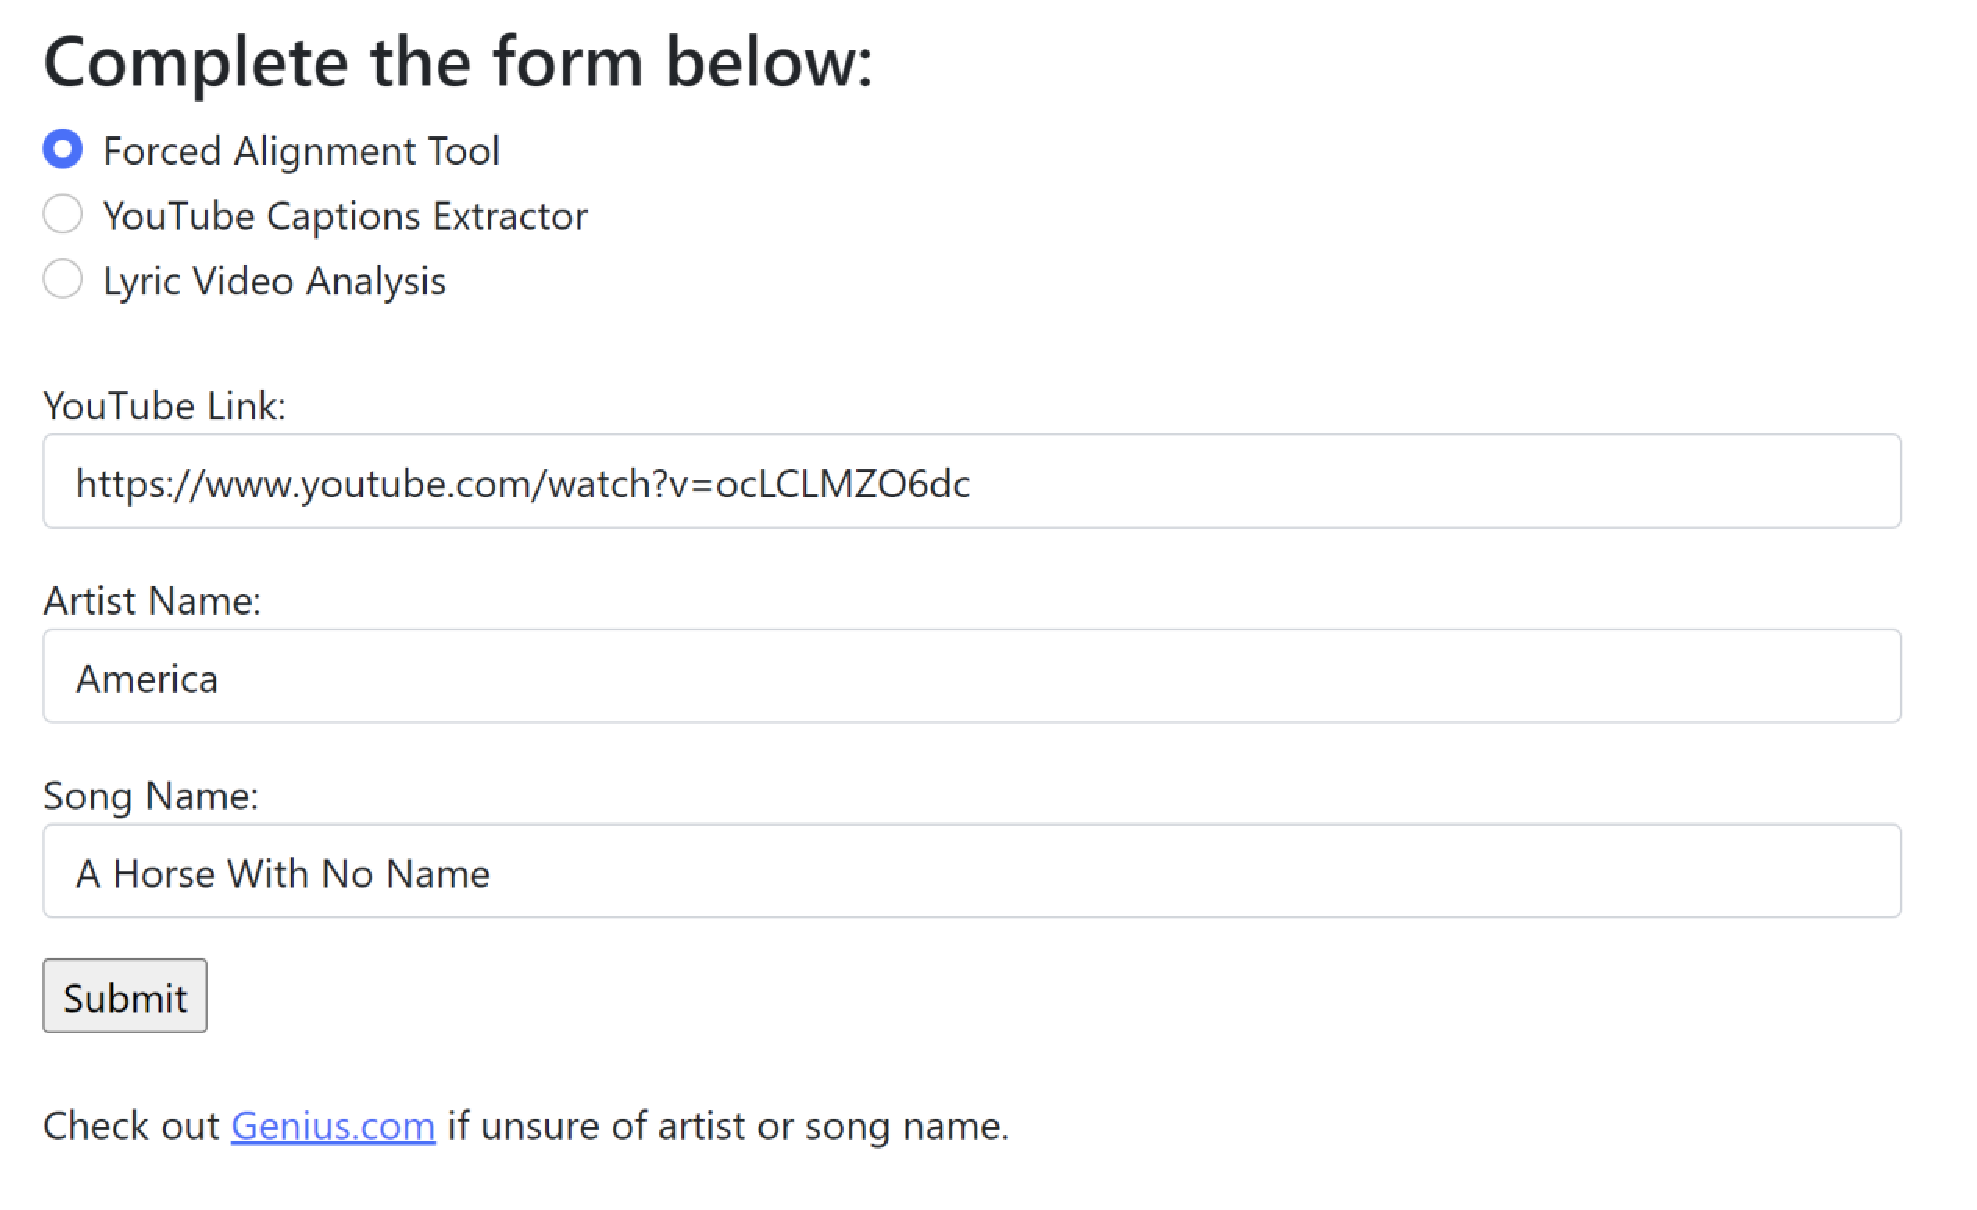
\includegraphics[width=0.8\textwidth]{figures/parker_interface.pdf}
    \caption{An example of using the user interface from the preceding system}
    \label{fig:parker_interface}
\end{figure}

\subsubsection{Problems}
Parker's system made many achievements in generating complementary videos for audio tracks. However, it was restricted to the YouTube platform and emerged with a number of unforeseen drawbacks.

\label{par:metadata_problem}
To begin with, the metadata of YouTube videos was deemed unreliable in procuring the artist's name and the song title. Therefore, the system resorts to obtaining this information from user input. However, this can be problematic since it requires the user to undertake additional research and accurately type the information, which can be prone to errors. 

The prior system was also heavily reliant on several Application Programming Interfaces (APIs) such as YAKE! for keyword extraction, pytesseract \citep{pytesseract} for OCR of frames, and Google Images for scraping images just to name a few. This places a high dependency on these APIs which may not be consistently maintained or may cause version conflicts with other packages. In fact, the AutoLyrixAlign API \citep{gupta2020ala}, utilised for the Forced Alignment approach has since been deprecated at the time of writing.

Additionally, the system suffered from recurring instances of irrelevant images being retrieved. This can be attributed to the disregard of the semantic context of the keywords during the search process. Furthermore, keywords with multiple meanings in the English language often yielded incorrect images.

The ultimate problem identified, which directly prompted our idea of ground truth construction, stemmed from the evaluation phase of the project. The user surveys exhibited a mixed, albeit predominantly favorable assessment of the system. Nevertheless, the significant variance in ratings and responses to the open-ended questions emphasised the arduousness of conducting qualitative evaluations on automated videography systems. Furthermore, such evaluations produced biased and non-repeatable outcomes.

\subsubsection{Improvements}
Now that the main problems have been identified, we must present solutions so that we can gather the appropriate requirements for this project. The first goal is to generalise the system to any type of audio. This involves not being restricted to English sources. Adding support for multiple languages would further our motivation for increased user accessibility to content. Moreover, this would allow easier content creation for many resource-poor languages.

First of all, let us tackle the metadata problem. We want to avoid relying on the user for metadata information for the audio source which means we must acquire this from somewhere else. This data was primarily used to query the Genius database in order to retrieve the lyrics transcription for songs so this data is not required for non-musical sources. Therefore, in order to identify the song title and artist, we could use the audio itself as the query. Shazam \citep{wang2006shazam} is an application that can recognise music and movies by listening to a short sample of the audio. It does this by attempting to match the audio's time-frequency signature to one stored in its large catalogue of audio fingerprints to get the correct track information. While this approach would mean an additional API, its benefits of increased automation outweigh the drawbacks.

In order to retrieve more relevant images, it is clear that semantics must be introduced instead of relying on keyword-based searching. Upon researching the recent advancements with CLIP (\ref{sec:background_clip}), we believe this is a viable solution that can mitigate the number of non-relevant images being retrieved.

Lastly, we believe our novel ground-truth annotation interface will address the difficulty of evaluating current and future automatic videography systems. The constructed relevance assessments allow for the application of the Cranfield paradigm and computing standard IR metrics. These quantitative measures permit impartial performance comparisons between different systems. More importantly, the experiments can be conducted rapidly and repeatedly without concerns about result consistency.


\subsection{Labelbox}
\label{sec:labelbox}
Labelbox is a cloud-based platform for data labeling and annotation. It is used by many companies to build and improve machine learning models. Founded in 2018, it offers a range of annotation tools including image classification, object detection, and segmentation. Its image classification tool allows users to label images with relevant tags or categories, such as "dog" or "cat". For our specific task, Labelbox allows users to query for specific concepts using natural language, which returns a ranked list of relevant images. The user can then select the most appropriate images by checking a box and saving them for export. An example of this process can be seen in Figure \ref{fig:labelbox_interface}, where an annotator marks relevant images for the concept, \emph{"painting of cocktails"}.

\begin{figure}[h]
    \centering
    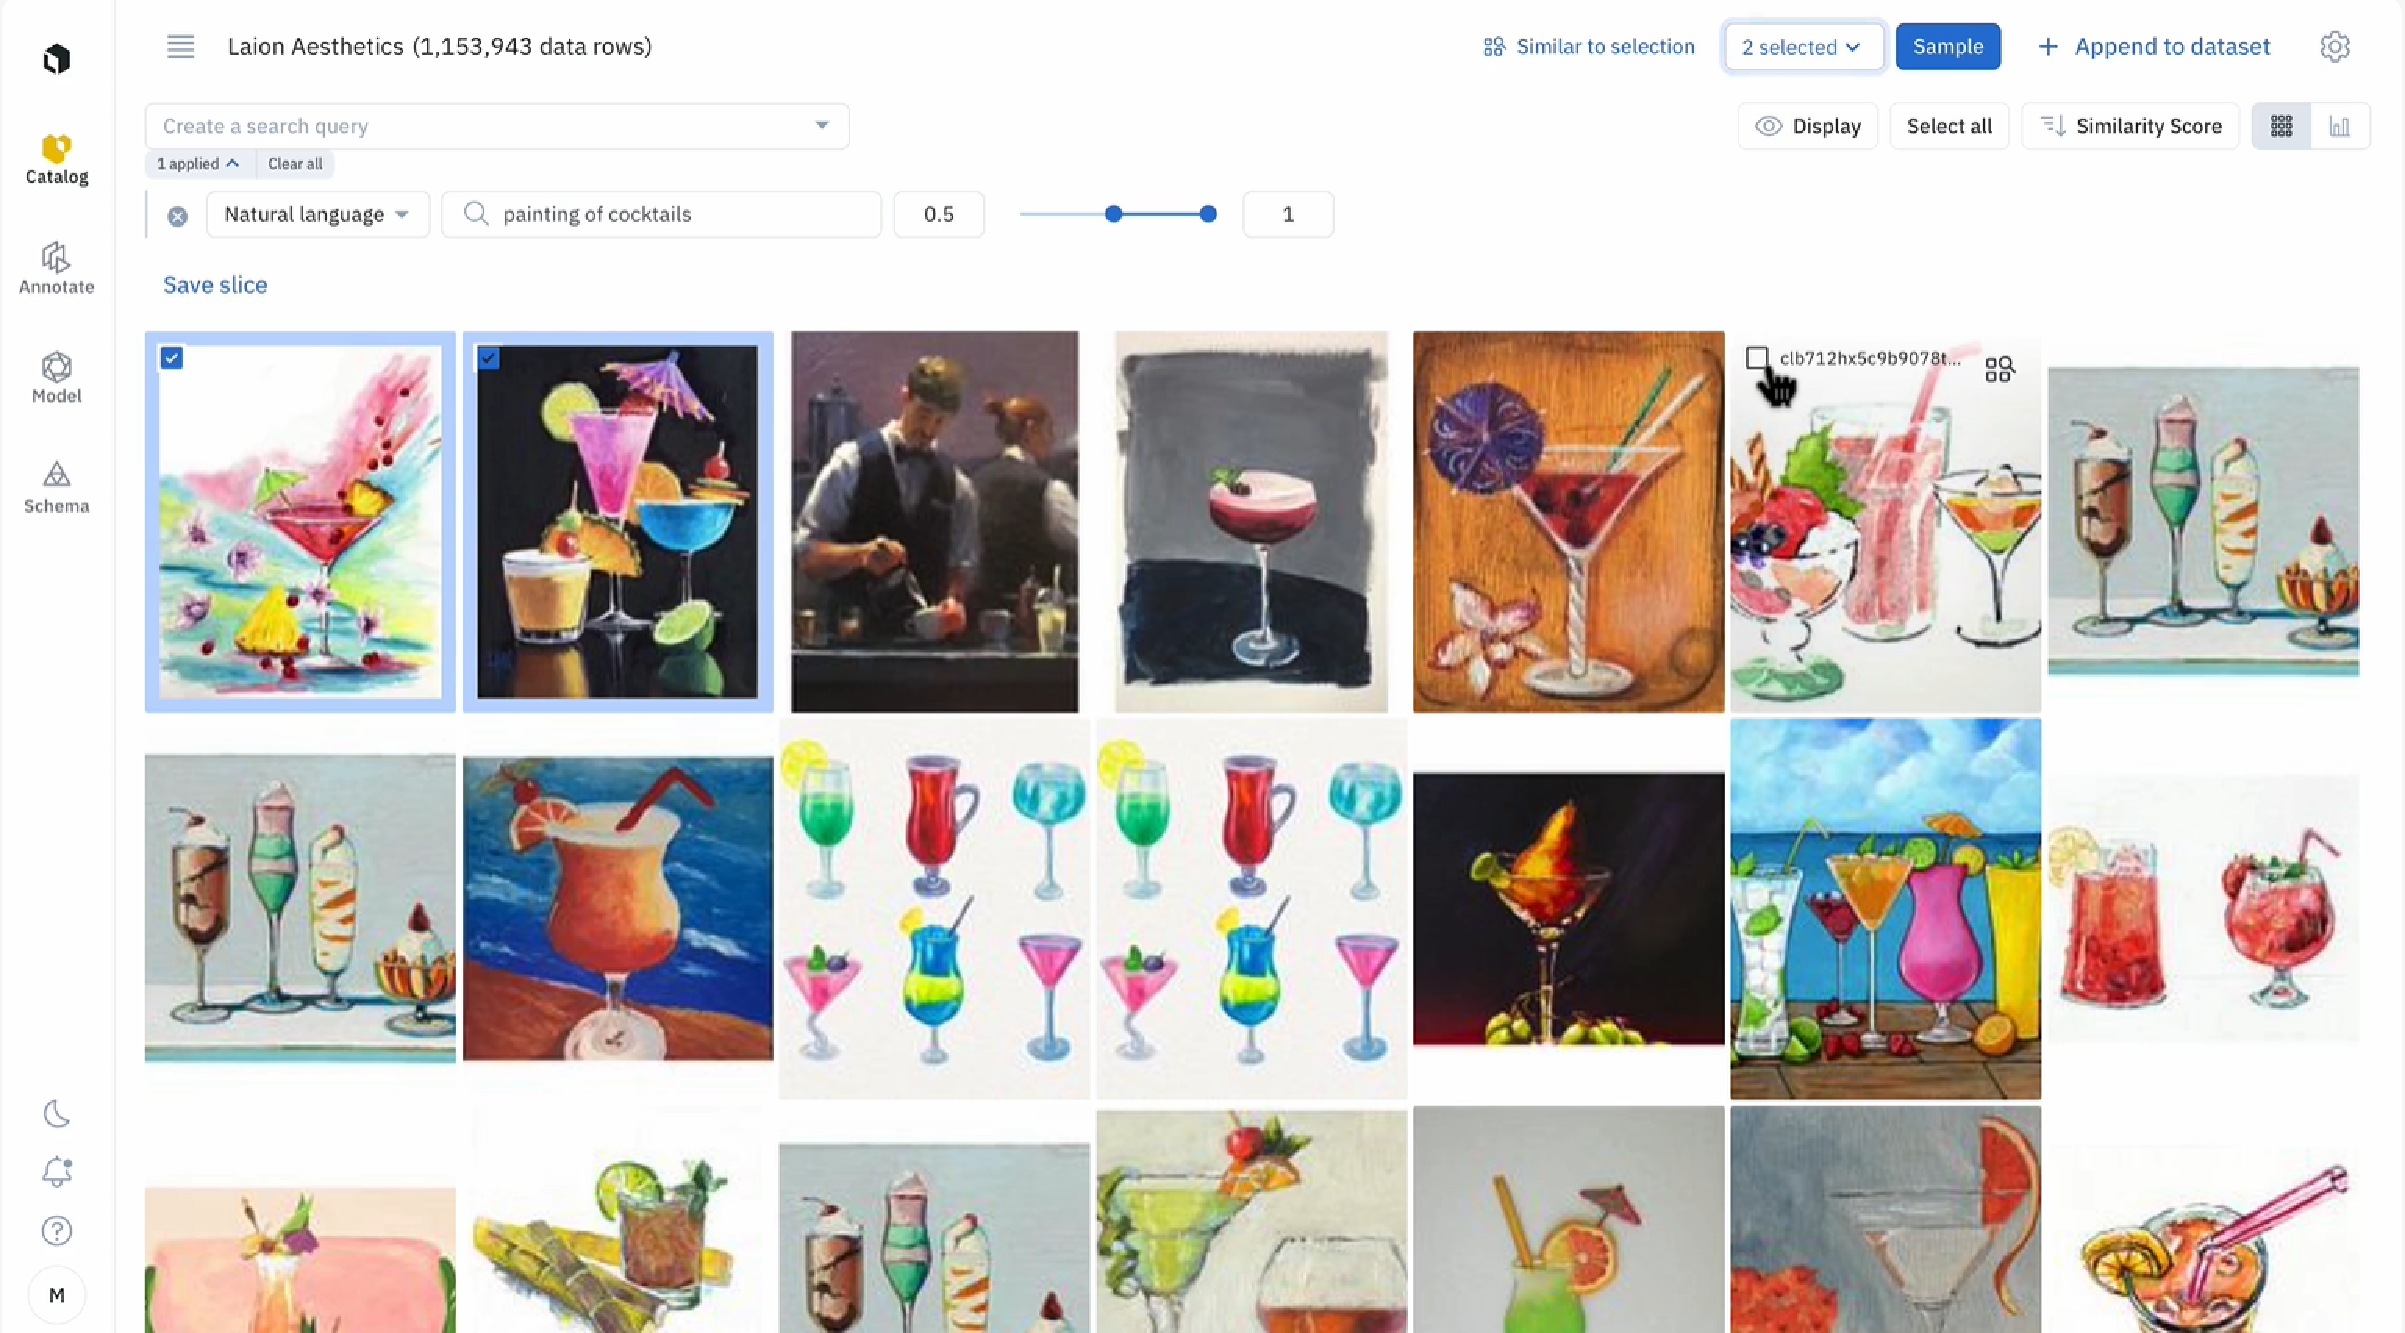
\includegraphics[width=0.9\textwidth]{figures/labelbox_interface.pdf}
    \caption{Relevance assessment of the concept "painting of cocktails" using the Labelbox interface}
    \label{fig:labelbox_interface}
\end{figure}

One of the most appealing features that Labelbox offers is allowing users to customise the embedding model for similarity searching and its aesthetic hyperparameter, as illustrated in Figure \ref{fig:labelbox_model}. Currently, Labelbox only supports the CLIP ViT-B/32 model for images. However, the platform is designed to be compatible with any model, which can be configured using their well-documented API.

\begin{figure}[h]
    \centering
    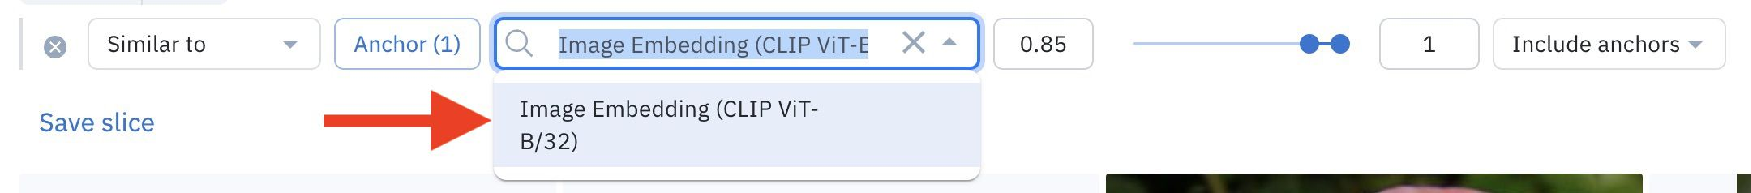
\includegraphics[width=1\textwidth]{figures/labelbox_model.pdf}
    \caption{Labelbox providing the option to customise the image-text embedding model}
    \label{fig:labelbox_model}
\end{figure}

The platform also integrates with popular machine learning frameworks and cloud services, allowing companies to streamline their data labeling workflows and accelerate model development. Despite the platform's slick design, getting acquainted with the application takes time, just due to the sheer multitude of available features and tools.


\subsection{SuperAnnotate}
\label{sec:superannotate}
Founded in 2017, SuperAnnotate is another cloud-based platform for computer vision and machine learning, designed to help users create high-quality image datasets for training and testing models. The platform allows the annotation of images with bounding boxes, polygons, or keypoints, among others, as well as the ability to collaborate with other annotators on the fly. The platform has since grown rapidly and has been used by companies and researchers across diverse industries including autonomous vehicles, medical imaging, and agriculture.

SuperAnnotate is not just restricted to images, it also offers tools for annotating audio, video, LiDAR and any custom data formats like PDFs or HTML. However, the platform's comprehensive feature set is only accessible via a paid subscription model, which may not be ideal for individuals who require a single tool such as image relevance assessing. Figure \ref{fig:superannotate_interface} depicts SuperAnnotate's interface to query images using natural language, similar to Labelbox (\ref{sec:labelbox}). The interface also allows placing tags in order to filter the retrieved images by specific attributes such as traffic lights that only show red. However, unlike Labelbox, SuperAnnotate does not provide an off-the-shelf embedding model, necessitating users to feed a model themselves.

\begin{figure}[h]
    \centering
    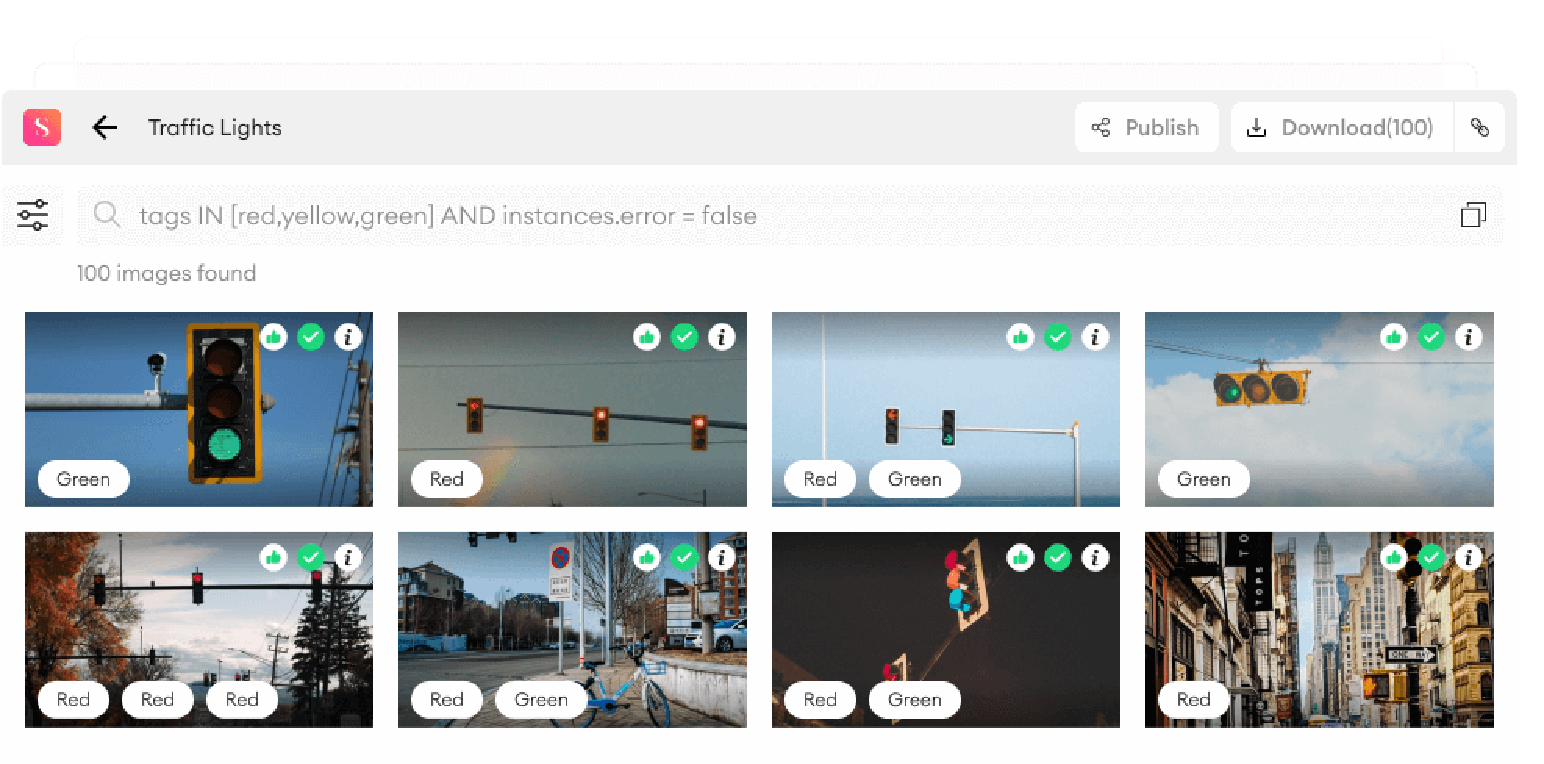
\includegraphics[width=1\textwidth]{figures/superannotate_interface.pdf}
    \caption{Relevance assessment of the concept "Traffic Lights" using SuperAnnotate's interface}
    \label{fig:superannotate_interface}
\end{figure}


% \section{The Bigger Picture}
% Exploring the background of the project through a review of the history and past accomplishments within the field is essential to establish its relevance and reason for existing. Looking at current solutions to the problem and their contrasting approaches provides valuable insight into which direction we take our project. Nevertheless, it is equally important to envisage the potential applications of our project beyond its primary focus of automated videography. For this reason, we look into recent research that aims to reduce relevance assessment efforts by employing query-specific variable depth pooling (CITE).


\section{Summary}
Exploring the background of the project through a review of the history and past accomplishments within the field is essential to establish its relevance and reason for existing. Looking at current solutions to the problem and their contrasting approaches provide valuable insights into the direction we should take our project. This is made explicit by our explorative dissection of the previous system as we propose potential solutions for its limitations. The advent of OpenAI's CLIP and Whisper \citep{whisper} models allow for a unique approach to the videography pipeline that could expand its current capabilities.

Regarding the annotation interfaces, both applications we reviewed share an intuitive interface design including clear checkmarks to indicate images tagged as relevant by the user. Nonetheless, even with the vast feature set that these systems offer, it still requires a lot of manual effort to complete the presented task in this project. To exemplify, the assessor must first listen and transcribe an audio source and subsequently input and annotate every segment within the transcript one by one. We believe our solution could streamline this procedure by automating the transcription process and making it easier to view and assess different audio segments within the interface itself.


%==================================================================================================
\chapter{Analysis/Requirements}
\label{chap:requirements}
This chapter serves to break down the high-level aims of the project in order to produce a list of functional and non-functional requirements, ordered by priority. This will directly determine the design and implementation of the project.

\section{Requirement Elicitation}
In order to elicit the list of requirements, a number of user scenarios are created. These are imagined scenarios of users that would directly benefit from such an application. This type of requirements gathering, most commonly used in agile software development projects, places the focus on the end-user, rather than the developer. Therefore, this prioritises the features that an end-user requires to fulfill their goals rather than designing the development process around what is easy to implement. Another benefit of this method is that it mitigates the risk of potential flaws at a very early stage. It is much easier to accommodate any flaws before any design or implementation is undertaken rather than finding them out during the evaluation stages with real users. It gets progressively more difficult to change the existing design the further we are down the development process.


\subsection{User Scenarios}
\subsubsection{User Scenario 1: Anna} is a young secondary school teacher who has started recording her classes in response to the recent shift in online learning. She regularly posts her recordings to an online platform supported by the school. However, she has had a few complaints from her students that her recordings are not engaging enough and that it is difficult to see what she writes on the board. Anna strives to provide the best for her students and wishes she could make her recordings more engaging by illustrating the concepts she talks about in her audio recordings. However, she does not know anything about video production and is worried about the time required to learn and edit videos daily. She wishes for a tool that automatically illustrates her audio recordings in a swift manner. The created video should include captions to make it as accessible as possible for her students.

\subsubsection{User Scenario 2: William} has recently built two new automated video generation tools that use differing reranking procedures to retrieve the top images from the text. He has performed some user studies, where he asked a number of users to watch and rate the videos generated by both systems on the same audio tracks. He used A/B testing in order to compare the performances of his two systems. However, the user studies resulted in very mixed results, with some users rating system $A$ highly while others rated system $B$ as better. Furthermore, upon closer inspection, he found that the user ratings varied wildly depending on the audio tracks present in the videos. This was problematic since the user studies took over 2 hours to complete and William is unwilling to conduct another when it is unclear if the results would even improve with new participants. William wished that he could objectively evaluate his systems against a fixed test collection of ground truths. He would be able to use this to obtain quantitative metrics for each system that he could compare giving a clear answer to which reranking procedure performs better.

\subsubsection{User Scenario 3: Lucy} is a software developer who is part of a small team who is building a new videography tool. Her manager has given her the tedious task of assessing the relevance of images for a predetermined set of audio from videos sourced from YouTube. This process requires manually annotating images that are the most fitting for the textual content existing within the audio. This is a very lengthy process since she must listen to the audio track multiple times in order to accurately transcribe the textual content. Following this, she must manually record the locations of the annotated images in a spreadsheet. Her manager has also assigned a colleague to double-check each annotation made. She wishes for a tool that automatically transcribes the audio and provides an easy-to-use interface to annotate relevant images. She requires that this ground truth could be downloaded in a human-readable format. Additionally, it would be helpful to be able to edit the annotations after the fact, so that her colleague can fix any incorrectly judged images.


\subsection{User Stories}
\begin{itemize}
    \item \emph{As a user} of the application, \emph{I want to} upload audio files, \emph{so that} I can generate a video from it or construct ground truths for it.
    \item \emph{As a user} of the application, \emph{I want to} specify YouTube video URLs, \emph{so that} its extracted audio can be used as the source.
    \item \emph{As a user} of the application, \emph{I want to} build and download the set of ground truths, \emph{so that} I can use them to evaluate my system.
    \item \emph{As an user} of the application, \emph{I want to} edit previously made ground truths, \emph{so that} I can fix any mistakes made.
    \item \emph{As a user} of the application, \emph{I want} to view the full audio transcription, \emph{so that} I can annotate specific parts of the audio.
    \item \emph{As a user} of the application, \emph{I want to} view and download the generated video, \emph{so that} I can share it and upload it to any platform.
\end{itemize}


\section{Requirements}
In order to formalise and prioritise the main requirements identified, the MoSCoW method \citep{clegg1994moscow} was chosen. While it would be desirable to develop every feature that could help achieve the project's goal, the project's limitations make it impractical. Therefore, it is crucial to assess each feature's importance by evaluating how much it would contribute to achieving the intended goal. Each feature will fall into one of four categories:

\begin{itemize}
    \item \textbf{Must Have:} These are essential features that must be implemented to fulfill the project's aim.
    \item \textbf{Should Have:} These features are highly desirable, but missing them will not directly lead to a project failure.
    \item \textbf{Could Have:} These are features that are beneficial but are viewed as extra perks.
    \item \textbf{Won't Have:} These features are not worth pursuing.
\end{itemize}

The list is divided into two sections: Functional Requirements, which describe interactive features, and Non-Functional Requirements, which describe program properties that users cannot interact with. Requirements marked by an \textbf{*} were added at later stages in the project development as new feature ideas emerged.

\subsection{Functional Requirements}
\begin{enumerate}
    \item \label{req:1} \textbf{Must Have:} The ability to upload an audio file as an input audio source.
    \item \label{req:2} \textbf{Must Have:} The ability to specify a YouTube video URL as an audio source.
    \item \label{req:3} \textbf{Must Have:} The ability to view the full audio transcription.
    \item \label{req:4} \textbf{Must Have:} The ability to generate an illustrated video for any audio source.
    \item \label{req:5} \textbf{Must Have:} The ability to view the top-$k$ retrieved images for a given audio chunk.
    \item \label{req:6} \textbf{Must Have:} The ability to annotate the most-fitting images for a given audio chunk.
    \item \label{req:7} \textbf{Must Have:} The ability to view the text present in a given audio chunk.
    \item \label{req:8} \textbf{Must Have:} The ability to view the constructed ground truth data.
    \item \label{req:9} \textbf{Must Have:} The ability to download the constructed ground truth data in a portable format.
    \item \label{req:10} \textbf{Should Have:} The ability to view previously processed audio sources, generated videos, and constructed ground truths.
    \item \label{req:11} \textbf{Should Have:} The ability to edit previously made ground truths.
    \item \label{req:12} \textbf{Should Have:} The ability to upload audio sources of any language.
    \item \label{req:13} \textbf{Could Have:} The ability to load ground truths for editing.
    \item \label{req:14} \textbf{Could Have:} The ability to reconfigure the static image collection location.
    \item \label{req:15} \textbf{*Could Have:} The ability to view the percentage complete for ground truth construction of processed audio sources.
    \item \label{req:16} \textbf{*Could Have:} The ability to save or skip chunks with repeating textual content when ground truth constructing.
    \item \label{req:17} \textbf{*Could Have:} The ability to view the timestamp information of audio chunks.
\end{enumerate}

\subsection{Non-Functional Requirements}
\begin{enumerate}[resume]
    \item \label{req:18} \textbf{Must Have:} The system using a static collection of images for repeatably consistent ground truth construction.
    \item \label{req:19} \textbf{Should Have:} The application being accessible from any Operating System platform.
    \item \label{req:20} \textbf{Should Have:} The application having a presentable user interface that is easy to use for any user.
    \item \label{req:21} \textbf{Should Have:} The application with appropriate error handling.
    \item \label{req:22} \textbf{Should Have:} The application displaying progress bars for long loading times.
    \item \label{req:23} \textbf{Should Have:} The application being fast and responsive.
    \item \label{req:24} \textbf{Should Have:} The system being able to recognise music tracks to automatically retrieve the artist name and song title.
    \item \label{req:25} \textbf{Should Have:} The application being able to provide a transcription for any audio source including phrase-level timestamps.
    \item \label{req:26} \textbf{Should Have:} The text-to-image retrieval system only retrieving relevant images by leveraging semantics of natural language as well as visual features.
    \item \label{req:27} \textbf{Should Have:} The videos being generated in a reasonable amount of time.
    \item \label{req:28} \textbf{Should Have:} The images being of high quality in the generated videos.
    \item \label{req:29} \textbf{Could Have:} The application being designed modularly to configure any static image collection.
    \item \label{req:30} \textbf{Could Have:} The videos including text as well as images.
    \item \label{req:31} \textbf{Could Have:} The application visually differentiating between previously processed audio sources.
    \item \label{req:32} \textbf{Could Have:} The system performing tempo or beat analysis to appropriately time image changes.
    
\end{enumerate}


\section{Summary}
This chapter presented a detailed outline of the essential features for the project's development. The approach involved crafting user scenarios and stories to gain insight into potential user needs, thereby deriving a MoSCoW prioritised list of requirements. This process provided greater clarity for the ensuing stage of the project - Design.

% What is the problem that you want to solve, and how did you arrive at it?
% \section{Guidance}
% Make it clear how you derived the constrained form of your problem via a clear and logical process. 

% The analysis chapter explains the process by which you arrive at a concrete design. In software 
% engineering projects, this will include a statement of the requirement capture process and the
% derived requirements.

% In research projects, it will involve developing a design drawing on
% the work established in the background, and stating how the space of possible projects was
% sensibly narrowed down to what you have done.

%==================================================================================================
\chapter{Design}
(TODO: REFERENCE REQUIREMENTS DIRECTLY)

This chapter serves to provide the initial design choices including a high-level view of the system workflow and the wireframes of the intended user interface. All decisions will be explained with a general aim to optimise the user experience and fulfill the identified system requirements. Next, a deeper look into the design choices of the internal workings of components. This allows our system to be implemented in any language while maintaining clean and agile software design principles. 

\section{High-Level Plan of System}
In order to start planning out the workflow of our system, it is necessary to simplify and abstract the key components that will make up the backbone of the system. Our system will be comprised of two sub-systems, an automatic videography tool, and a ground-truth annotation tool. However, both sub-systems will use the same underlying pipeline. The simplified workflow diagram displayed as Figure \ref{fig:simplified_workflow} shows the basic, black-boxed components that will make up our pipeline: a transcription extractor, a video generator, and an annotation interface.

The user will input an audio source which will be processed to extract a synced transcription of the audio content. Next, the user will have the option to either choose to generate a video or start constructing the ground truth for it. Each option will produce an output that the user can subsequently view and export. In line with the requirements, these outputs will be saved to the database for future editing.

\begin{figure}[h]
    \centering
    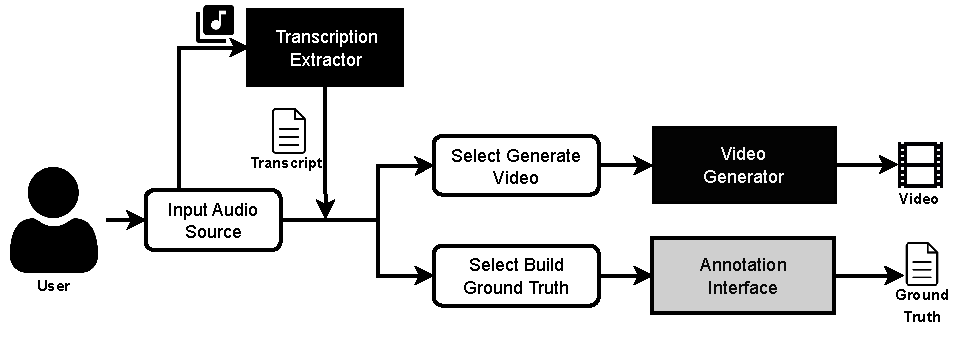
\includegraphics[width=1\textwidth]{figures/simplified_architecture.pdf}
    \caption{Simplified workflow diagram showing the basic high-level design of our system}
    \label{fig:simplified_workflow}
\end{figure}

\subsection{Transcription Extractor}
Firstly, the user will input an audio source. As stated in the requirements, this can either be in the form of a YouTube video URL or a direct upload of an audio file. This input will be passed along to the Transcription Extractor. This component will produce a transcription of the audio with phrase-level timing information. It is vital that this transcription is synced accurately with the audio since this information will be used to place relevant images during the video compilation.

There are a number of ways to retrieve the synced transcription, firstly, we can leverage YouTube's captioning system if the user chooses to input a YouTube video URL. We cannot always rely on this since captions are not guaranteed to be present. Secondly, for music, it is possible to retrieve synced lyrics from open-source databases, however, this would require identifying the artist name and track title. In order to avoid the YouTube metadata problem from the previous thesis \ref{par:metadata_problem} and allow this to function if the user uploaded an audio file, we must process the audio to recognise and retrieve the track information. Finally, we still require a backup audio transcription tool for non-music audio sources or containing no YouTube captions. This workflow is depicted in Figure \ref{fig:transcription_extractor}.

\begin{figure}
    \centering
    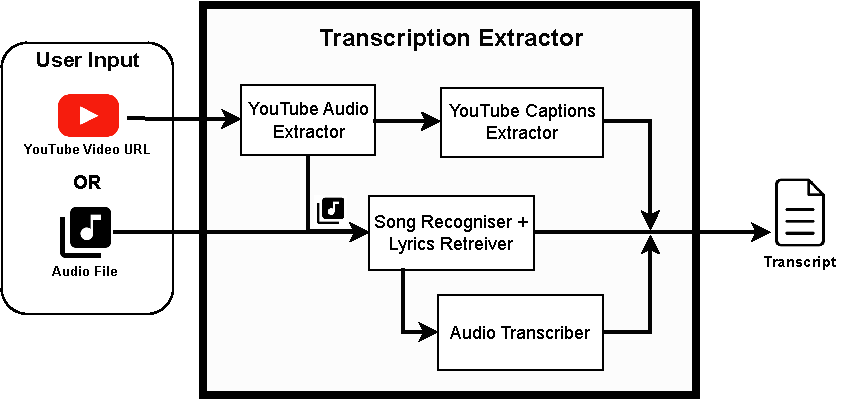
\includegraphics[width=0.8\textwidth]{figures/transcription_extractor.pdf}
    \caption{Internal view of the Transcription Extractor component}
    \label{fig:transcription_extractor}
\end{figure}

\subsection{Video Generator}
This component should activate when the user chooses to generate a video. It will take in the audio and the synced transcription which will be divided into phrase-level chunks. Now, the videography tool should retrieve a top-$1$ relevant image for each chunk and sequence them into a video according to the timestamp information present. The audio should then be added to this rendered video which will subsequently be outputted for the user to view and export. Since, it is common for some phrases to be repeated, especially in music, we may want to retrieve different images for each repeated phrase. Our main goal is to produce a video that is engaging to the user. In these cases, we can simply retrieve the next relevant image in our collection.

\subsection{Annotation Interface}
The Annotation Interface will consist of a system workflow of its own since the user will be actively interacting with the interface in order to incrementally construct the ground truth for the audio. Figure \ref{fig:annotation_interface} presents the workflow that an annotator would follow.

\begin{figure}[h]
    \centering
    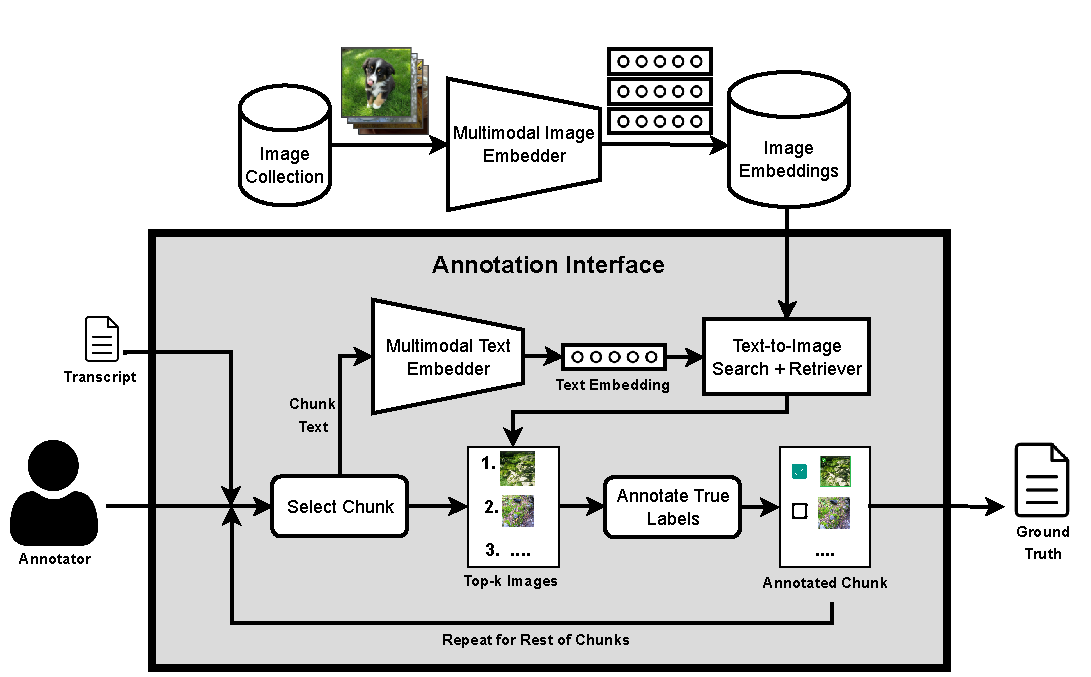
\includegraphics[width=0.95\textwidth]{figures/annotation_interface.pdf}
    \caption{Internal view of the Annotation Interface architecture}
    \label{fig:annotation_interface}
\end{figure}

Since one of our requirements specifies a static image collection (\textbf{\#\ref{req:18}}), this gives the benefit of being able to pre-process the entire collection since we know that the images are not going to change. Additionally, since we want to include the semantics of text and images, we must embed all the images into a multimodal space in which text can also be embedded into.

Firstly, the annotator would select an audio chunk to assess. This freedom to choose which part of the audio to annotate is essential in order to facilitate the requirement of editing annotations (\textbf{\#\ref{req:11}}). However, it can be assumed that the annotator will construct the ground truth in the order of the audio. Once a chunk is selected, the top-$k$ images will be retrieved and shown to the assessor by embedding the chunk text and performing a search in the multimodal vector space. The annotator is then expected to identify and label the images that they judge as the most fitting to the chunk text. This process will be repeated for every chunk of the audio until a completed ground truth set is constructed which will be outputted to the annotator in an accessible format.


\section{User Interface Design}
The user interface (UI) became a critical part of our application due to its importance within our task specification. Hence, ensuring our design was intuitive even for untrained users, to enable the freedom to crowdsource proved to be a challenge. Competing in the field with major annotation platforms only mounted more incentive to design an interface that is unique yet familiar. Furthermore, it was important to ensure pages within the UI remained uncluttered. For this reason, before any development started, we started prototyping interface designs using \cite{figma}.

\subsection{Home Page}
The simplified workflow outlined in Figure \ref{fig:simplified_workflow} will be used as the basis to form the various pages within the application. Firstly, we require a page for the user to enter the audio source to initiate the process. Hence, this 'home' page will require a way for the user to upload an audio file from their local machine (\textbf{\#\ref{req:1}}), as well as a text field to take in a YouTube video URL (\textbf{\#\ref{req:2}}). Appropriate validation is necessary to handle erroneous inputs such as incompatible file formats or URLs not from the YouTube domain. More importantly, these errors should be clearly displayed to the user so that they can respond accordingly. An initial design of the Home page can be seen in Figure \ref{fig:home_page}. 

In addition to taking inputs from the user, we also include a navigation bar with intended links to an 'About' page and a 'Collecions' page. Since we want our application to be open to anyone wanting to generate videos or develop ground truths, we believe an About page is necessary to provide information about the interface and how to use it. The link to a Collections page spawned to satisfy the potential to save processed audio sources and generated videos (\textbf{\#\ref{req:10}}). Furthermore, since these links are required to be easily accessible, we include this navigation bar on subsequent pages.

\begin{figure}
    \centering
    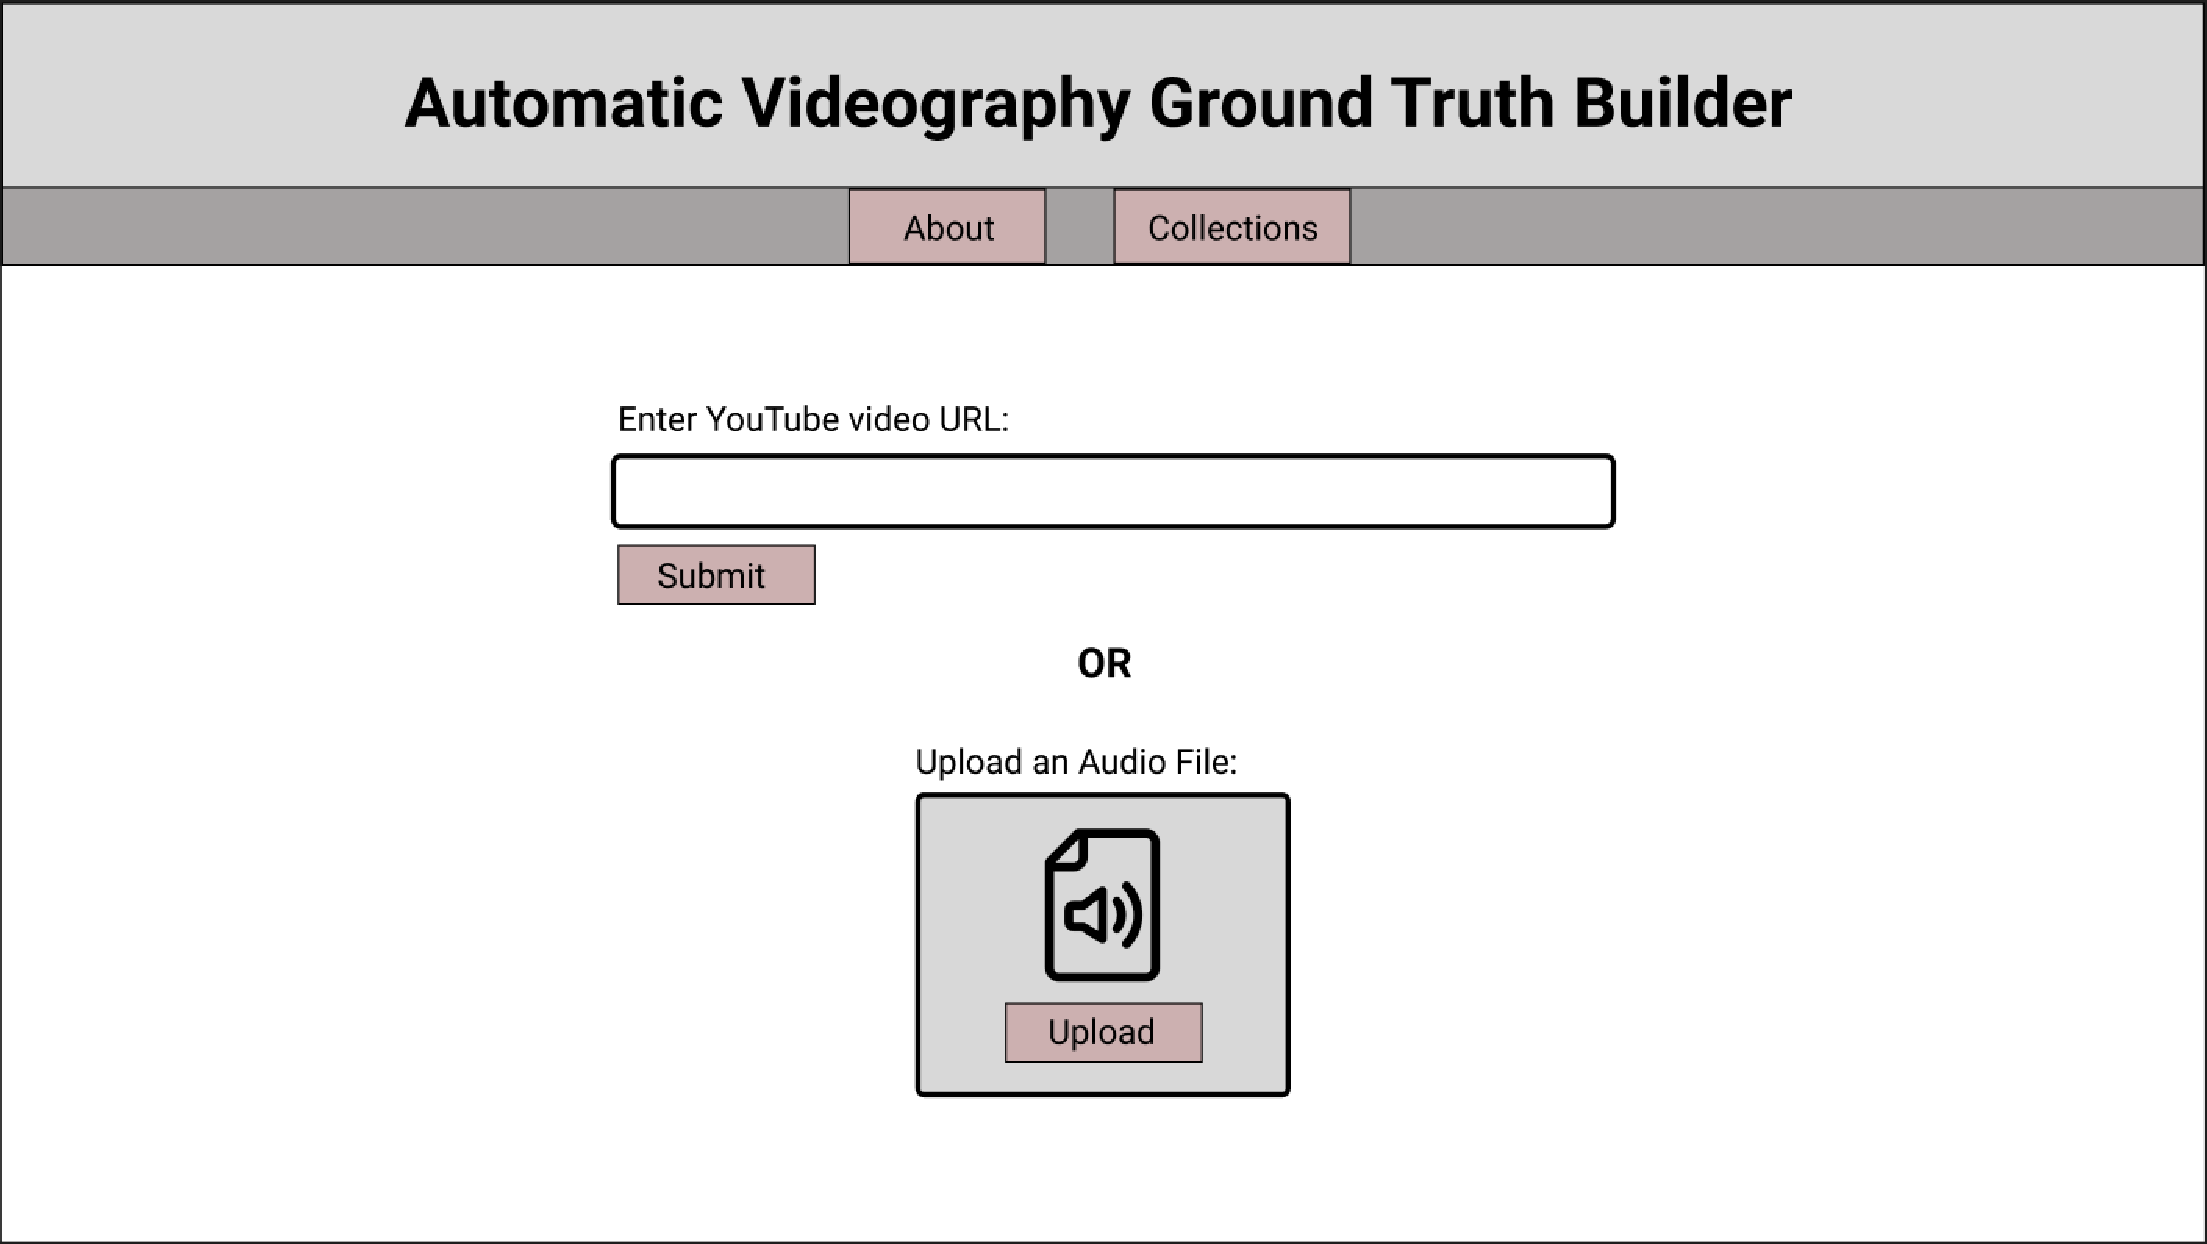
\includegraphics[width=0.95\textwidth]{figures/home_page.pdf}
    \caption{An initial prototype for the Home page, illustrating how the user can input an audio source.}
    \label{fig:home_page}
\end{figure}

\subsection{Audio Page}
Once the audio source is submitted, the Transcription Extracter component should produce a full transcription of the audio. This should lead into the next page displaying the results of the audio processing with the two different options of where to proceed next. More specifically, the user can choose to generate the video with the 'Generate Video' button, or start constructing a ground truth with the 'Build Ground Truth' button. The full transcription should also be shown to fulfill requirement \textbf{\#\ref{req:3}}. 

Aside from this, to save the audio processing result in a database, it must be uniquely identifiable. This led to the idea of associating the audio source to a Title and an optional Author. In the case where the audio is sourced from a file uploaded by the user, the title can simply be the filename. Whenever the audio is extracted from a non-music YouTube video, the title and author can be taken from the YouTube metadata. Finally, for music tracks, the title and author fields can be filled with the recognised track information such as the song title and artist name respectively. Our design shown in Figure \ref{fig:audio_page} also includes an associated image since we believe this could be visually appealing and satisfy the requirement to be able to differentiate collected audio sources (\textbf{\#\ref{req:31}}). This could simply be the video thumbnail for YouTube sources while for music tracks, the image field can be satisfied by its corresponding cover art. 

\begin{figure}
    \centering
    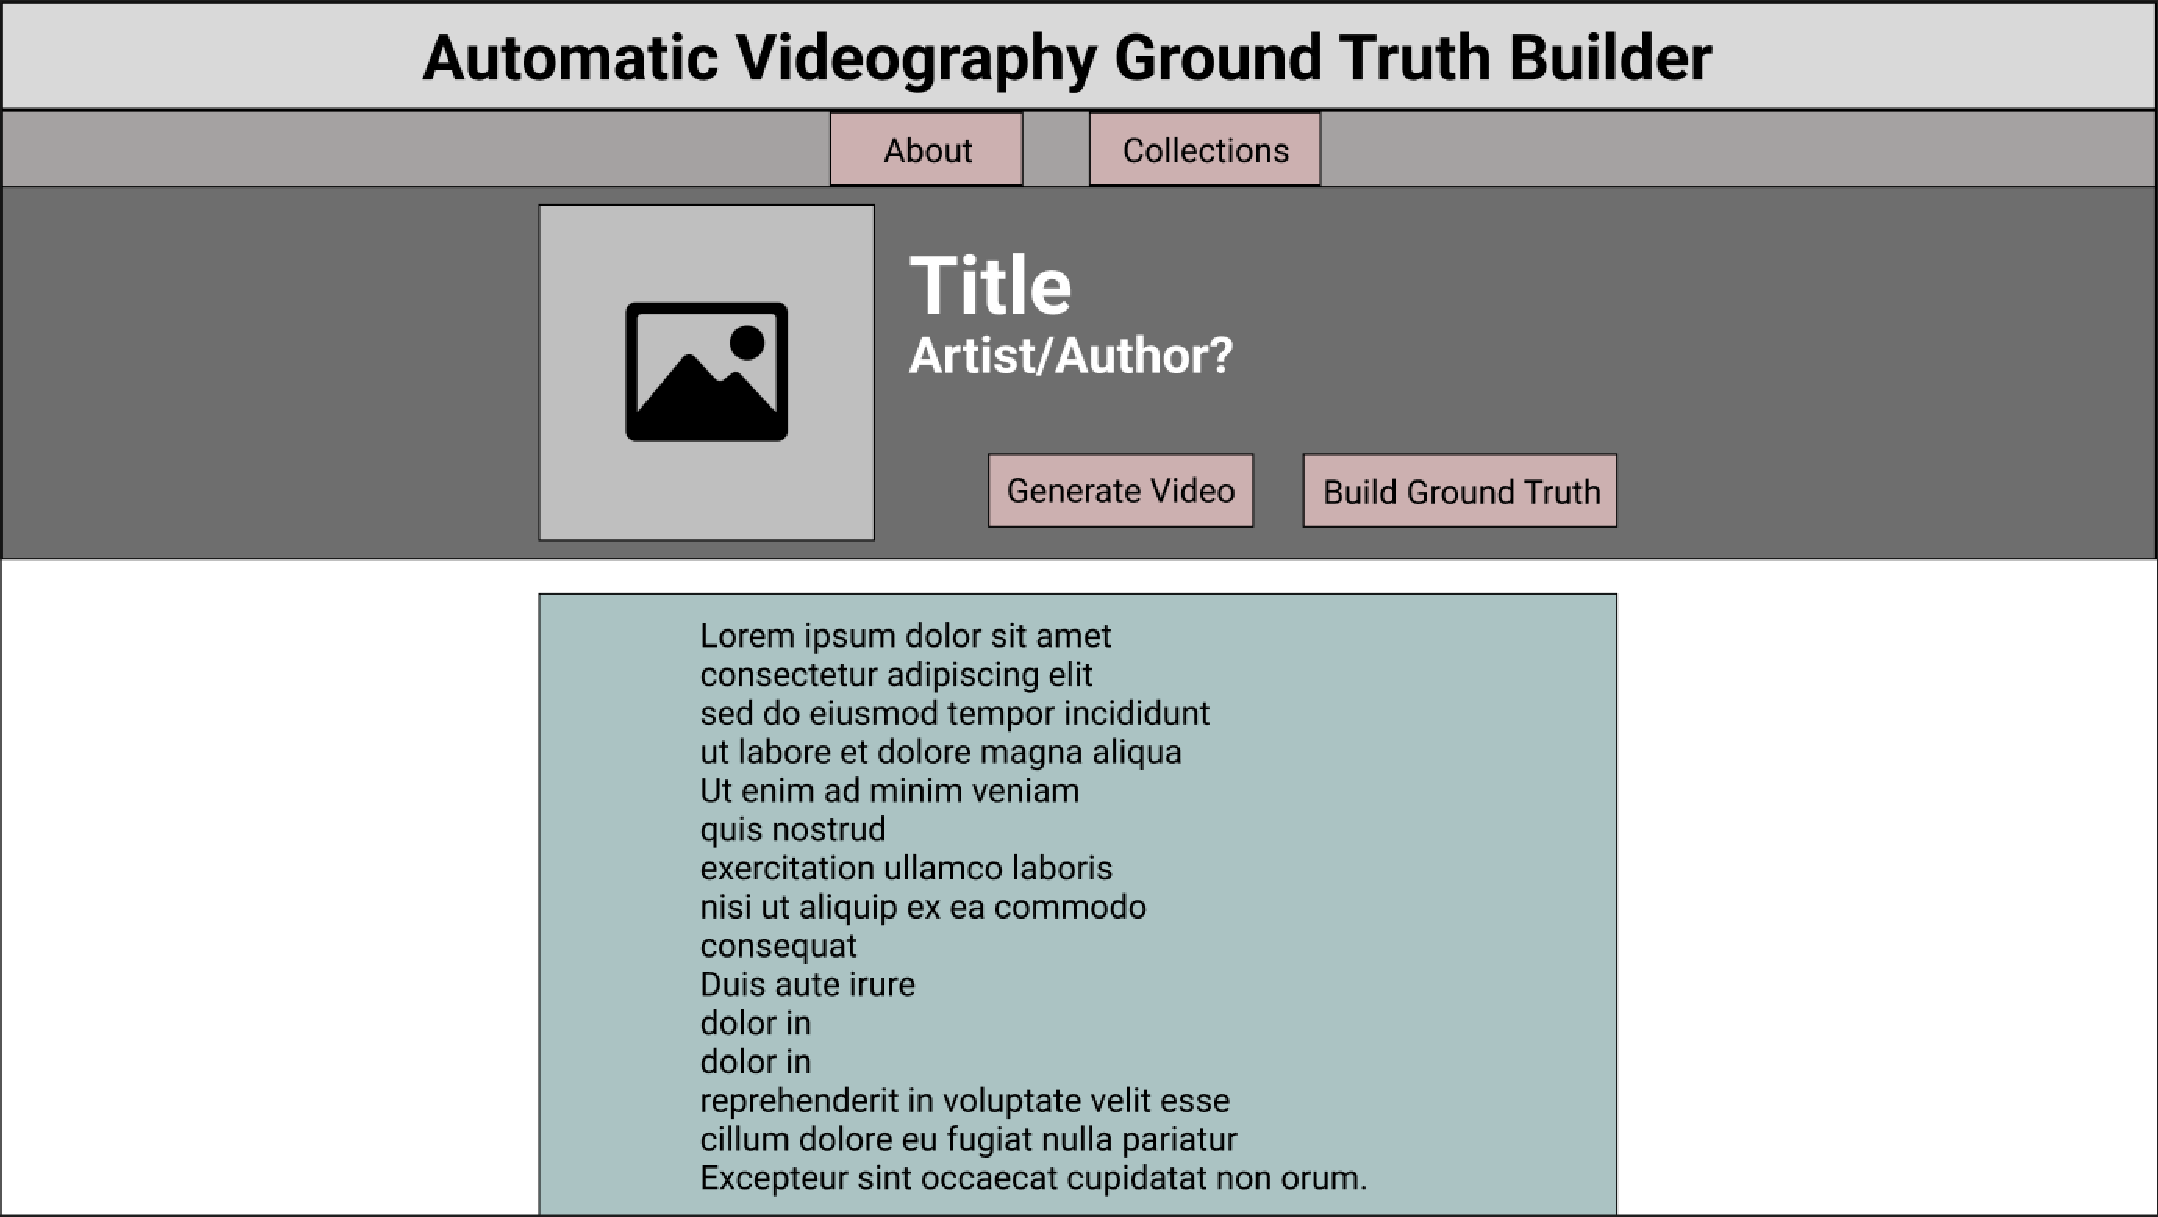
\includegraphics[width=0.95\textwidth]{figures/audio_page.pdf}
    \caption{An initial prototype for the Audio page showing the resulting transcript after processing the audio.}
    \label{fig:audio_page}
\end{figure}

\subsection{Video Page}
The Video page will be rendered when the user clicks on the 'Generate Video' button from the Audio page. This page will provide an embedded video so that the user could view the video on the interface itself instead of forcing them to download to view it. This page will be minimalistic in design, as illustrated in Figure \ref{fig:video_page}, and the 'Author - Title' divider will be utilised as the link back to the Audio result page. Once the video is generated, this will be saved in the backend for easy access. Prior to the rendering of this page, we intend to provide a descriptive loading screen since it is expected that the video compilation will take several minutes as made evident by the previous system. This intermediate loading page adheres to our listed requirements (\textbf{\#\ref{req:22}}) giving an estimated time of completion while simultaneously preventing the user from interacting with other parts of the interface during video generation.

\begin{figure}
    \centering
    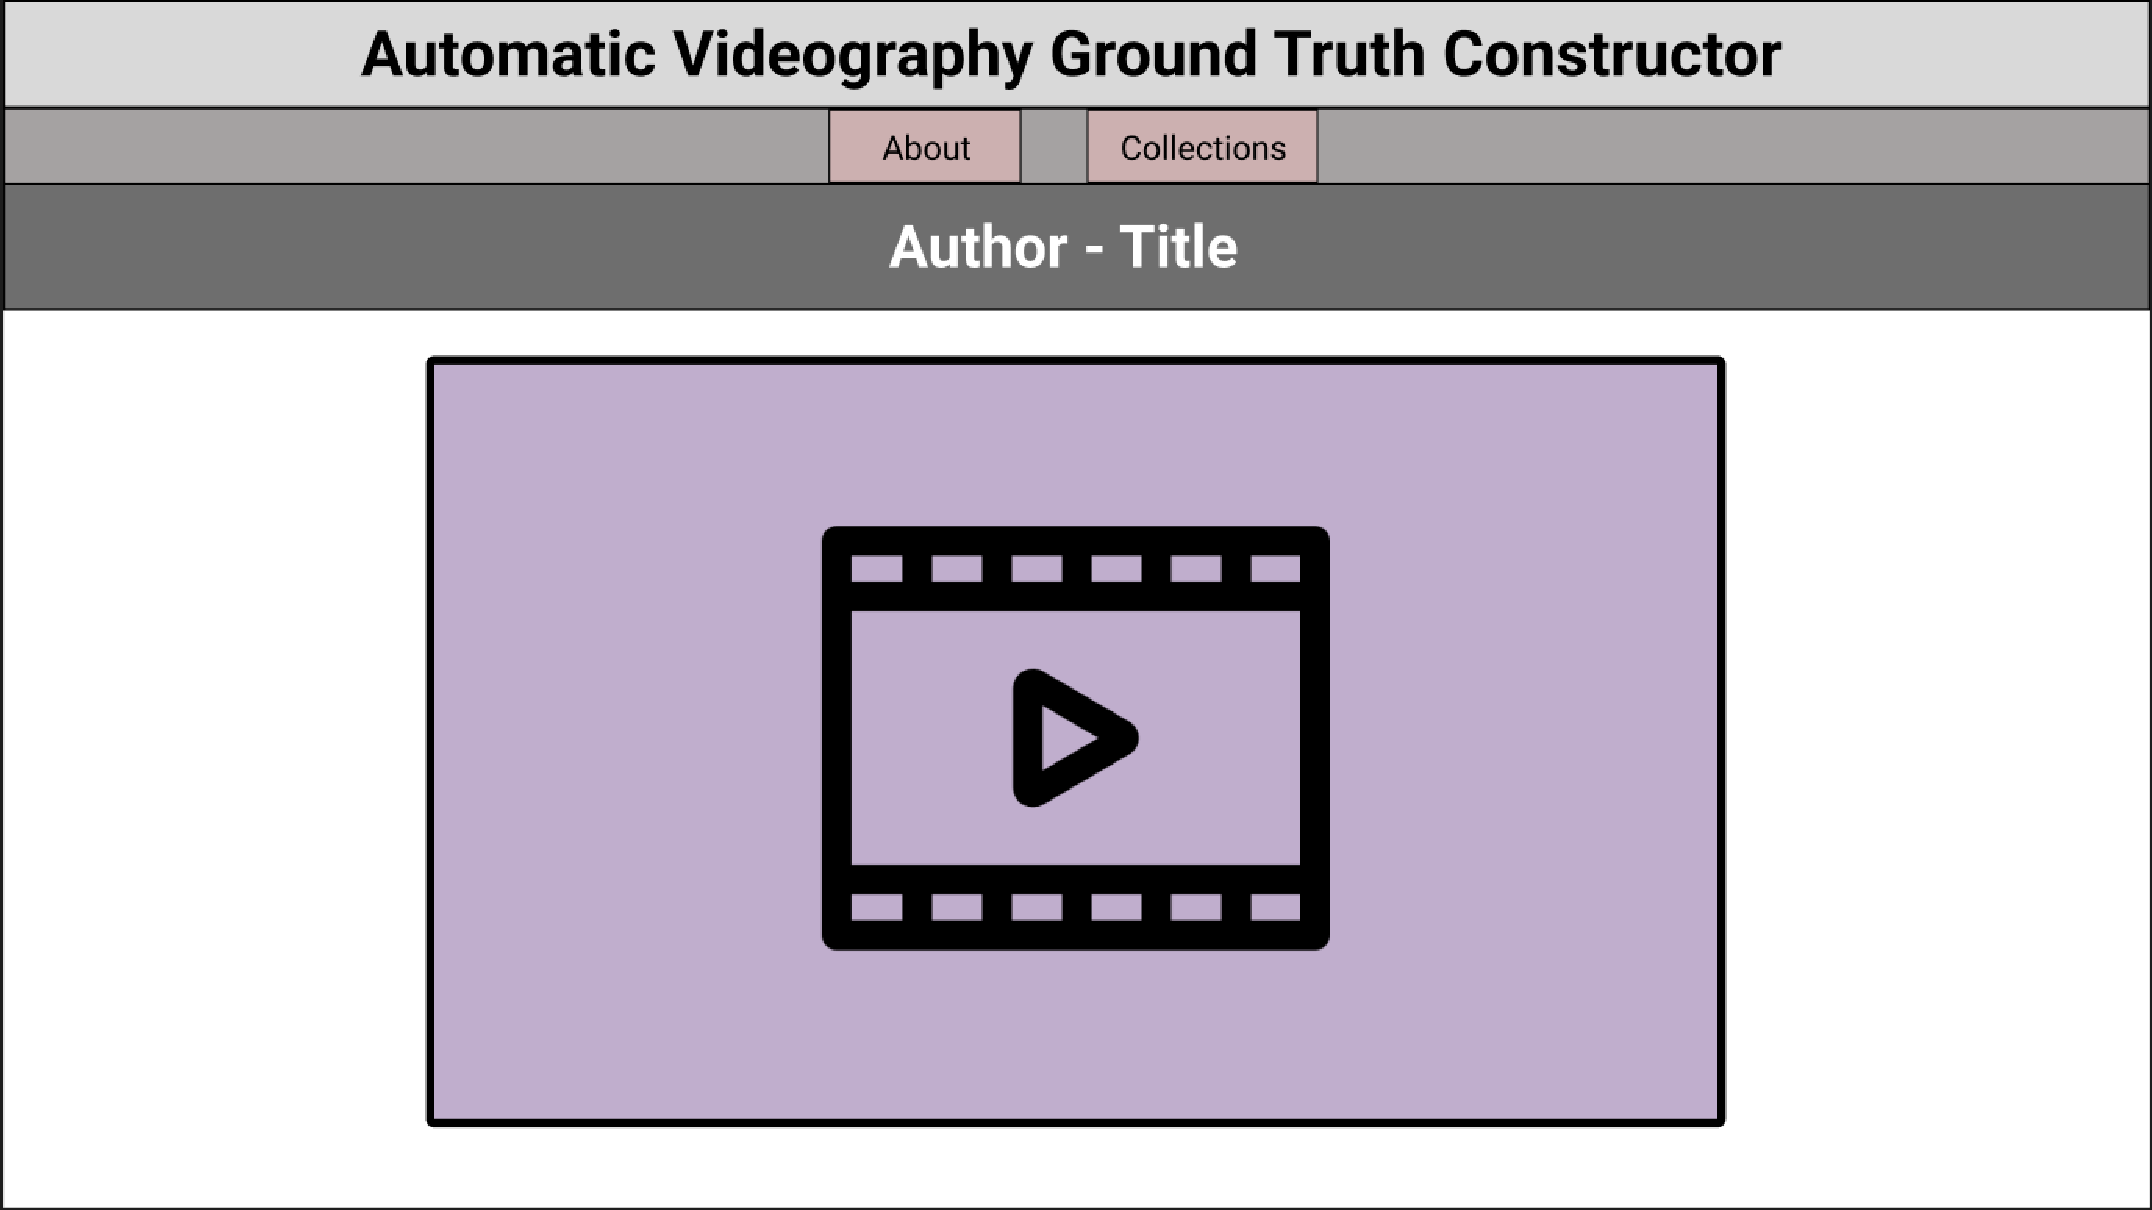
\includegraphics[width=0.95\textwidth]{figures/video_page.pdf}
    \caption{An initial prototype for the Video page providing the generated video.}
    \label{fig:video_page}
\end{figure}

\subsection{Chunk Page}
Alternatively, the user can choose to construct the ground truth for the audio source by clicking on the 'Build Ground Truth' button on the resulting Audio page. This should subsequently navigate the user to the first audio chunk page. This should show the text present within that chunk and the retrieved top-$k$ images using the system (\textbf{\#\ref{req:5}}, \textbf{\#\ref{req:7}}). As seen in Figure \ref{fig:chunk_page}, we picked a depth $k=10$ since it is small enough for the assessor to efficiently comb through for the most relevant images. This is especially true when this task must be repeated for every chunk in the audio source. We want to avoid a burdensome experience that could affect the quality of relevance assessments (CITE). However, we found that this cut-off point is highly dependent on the effectiveness of the retrieval system and the textual query discussed in the Implementation (REF).

\begin{figure}
    \centering
    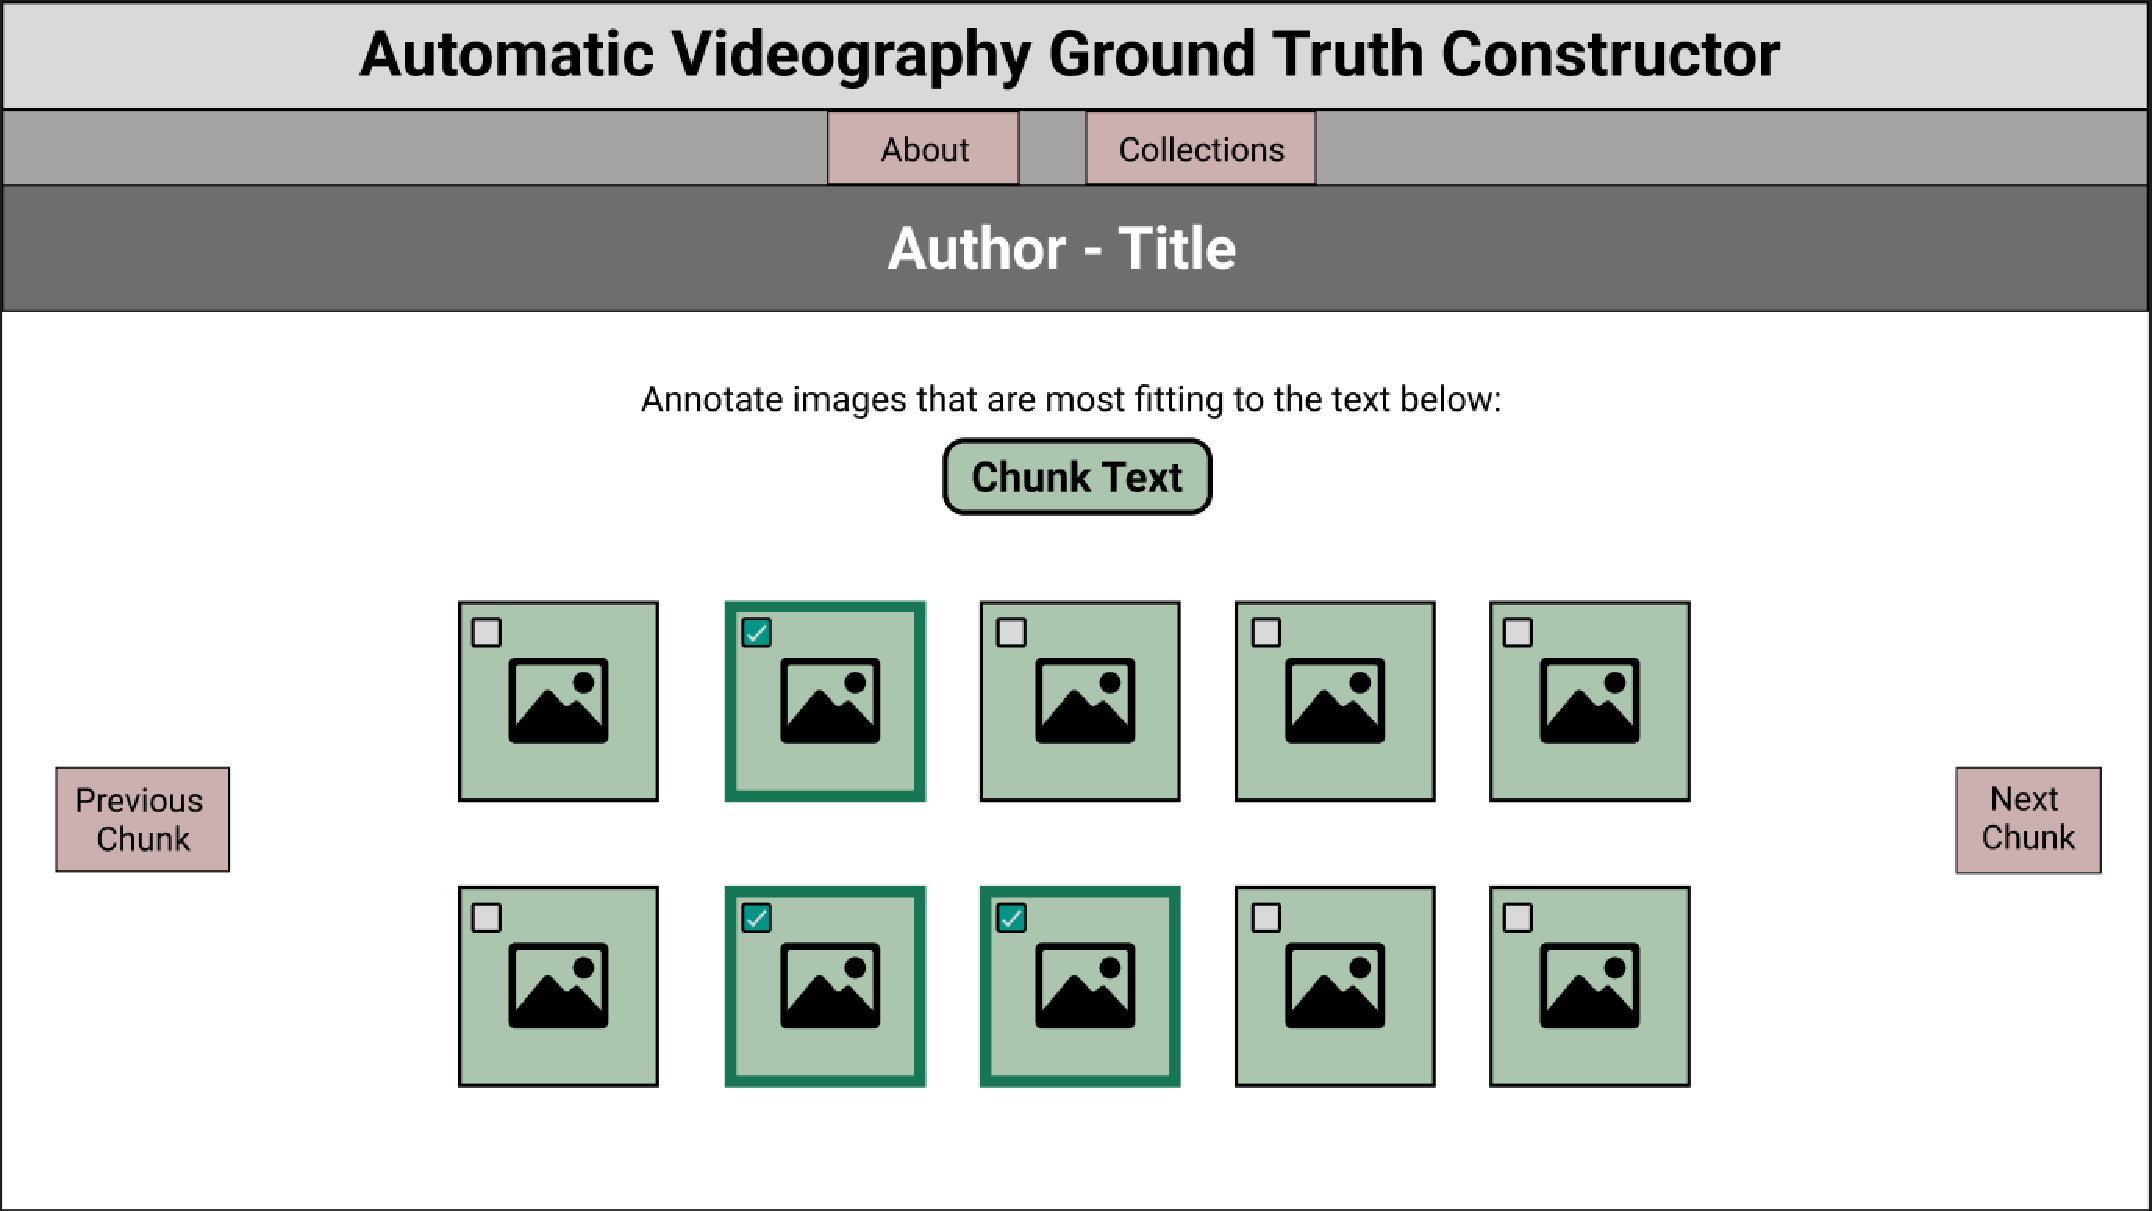
\includegraphics[width=0.95\textwidth]{figures/chunk_page.pdf}
    \caption{An initial prototype for the Chunk pages that provide the ability to assess the relevance of retrieved images for specific audio chunks.}
    \label{fig:chunk_page}
\end{figure}

We chose to use a binary relevance assessment strategy where the assessor must only mark relevant images meaning unmarked images are considered irrelevent (\textbf{\#\ref{req:6}}). This is faster than a graded relevance system which requires significant thought which may discourage accurate assessments. This is also backed by approaches employed by similar technologies (\ref{sec:labelbox} \& \ref{sec:superannotate}). However, it does call in question of what the assessor should do if all top-10 images are irrelevant to the chunk text, this is discussed in (REF). In addition to these interactive images, the page includes 'Previous' and 'Next' buttons to easily navigate to bordering chunk pages. We also intend to save the user's assessments when these buttons are pressed in order to reduce annotation effort and allow editing of previous chunks (\textbf{\#\ref{req:11}}). Not to mention to allow the possibility of skipping chunks with repeating textual contents (\textbf{\#\ref{req:16}}).

\subsection{Ground-Truth Page}
Once all audio chunks have been annotated, the system should render a resulting Ground-Truth page similar to Figure \ref{fig:ground_truth_page}. This will consist of a small preview of the ground-truth data and some functionality to download the constructed data (\textbf{\#\ref{req:8}}, \textbf{\#\ref{req:9}}). While the ground-truth data may be technical, we intend to deliver it in a human-readable format so that assessors can perform last-minute checks if required. The preview feature also enables retrieval system designers to peek at the format of the ground truths to aid in the evaluation process.

\begin{figure}[H]
    \centering
    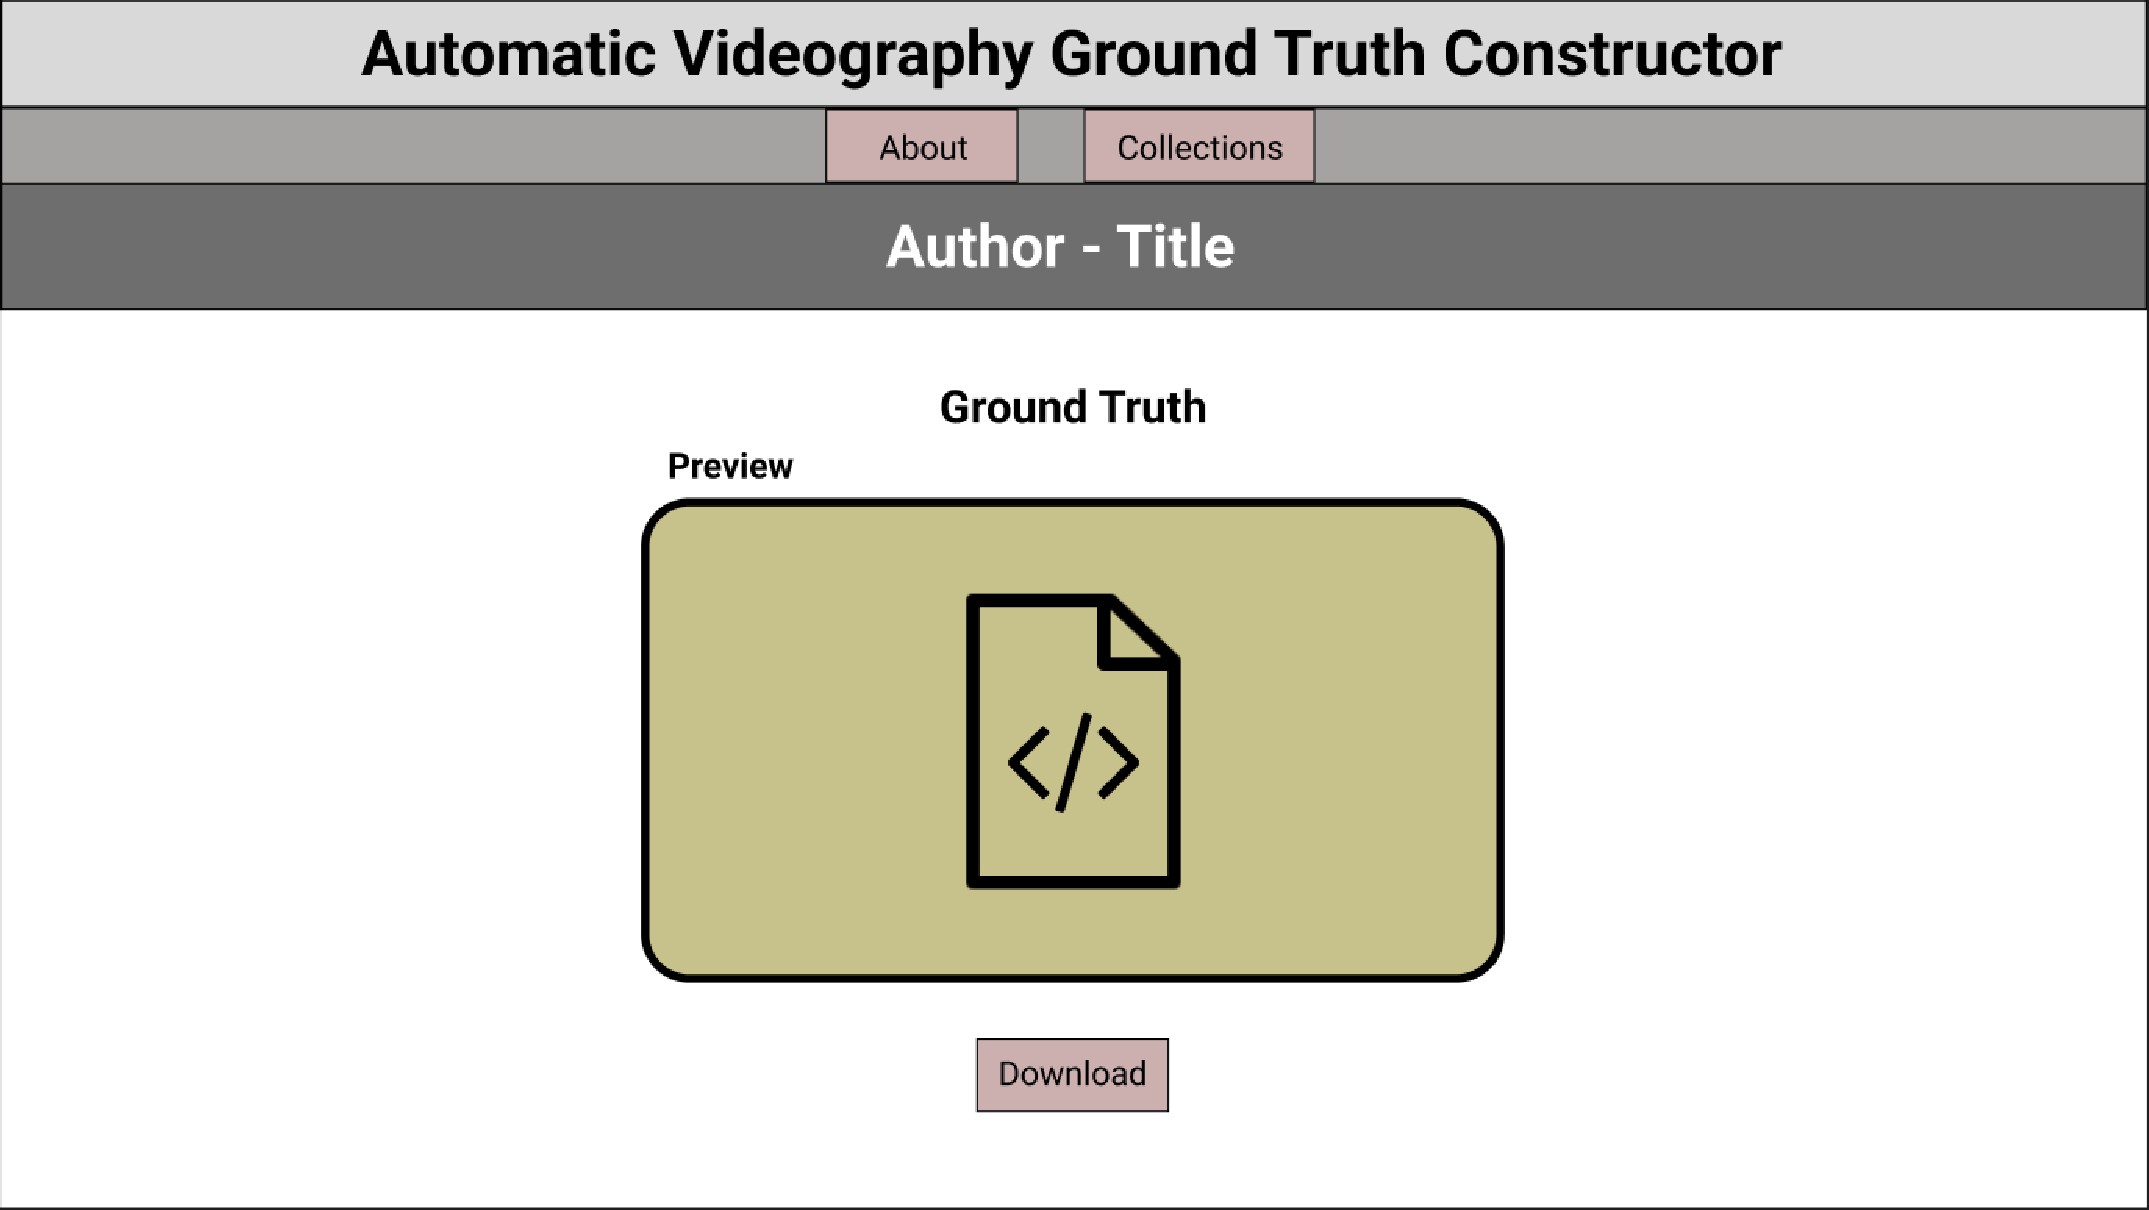
\includegraphics[width=0.95\textwidth]{figures/ground_truth_page.pdf}
    \caption{An initial prototype for the Ground-Truth Page providing a preview of the constructed ground truth available for download.}
    \label{fig:ground_truth_page}
\end{figure}


\section{Summary}
This chapter provided a comprehensive overview of the design choices made across all areas within the project. From the system architecture to the high-level decisions of the user interface following best Human Computer Interaction (HCI) design practices. Now that a detailed plan is in place, an intuitive entryway into actually implementing the project is uncovered, in a way that aligns with the requirements specification made in Chapter \ref{chap:requirements}. 

% How is this problem to be approached, without reference to specific implementation details? 
% \section{Guidance}
% Design should cover the abstract design in such a way that someone else might be able to do what you did, 
% but with a different language or library or tool. This might include overall system architecture diagrams,
% user interface designs (wireframes/personas/etc.), protocol specifications, algorithms, data set design choices,
% among others. Specific languages, technical choices, libraries and such like should not usually appear in the design. These are implementation details.


%==================================================================================================
\chapter{Implementation}
This chapter will provide a detailed look into the implementation of the project. The rationale behind all technology choices and their involvement to achieve our desired product will be explained here. 

\section{Software Development Process}
\subsection{Version Control}
\cite{github} was the chosen technology to host the remote copy of the repository and version controlling throughout the implementation. This ensured all code was regularly backed up, providing a layer of security against local data loss or corruption. In addition, it provided a detailed tracking of the project's development, allowing the freedom to go back to previous versions if necessary. Since this was an individual project every feature was developed sequentially making branching unnecessary due to the lack of potential merging conflicts. However, branching was utilised at the beginning of the project when it was unclear which direction the project should be taken. For instance, several options for the image collection were considered, most notably taking them from the \cite{wikimedia_commons} or \cite{imagenet}, each stored in separate branches.


\subsection{Application Framework and Language Choice}
It was decided the project should be developed as a web application due to the system requirement \textbf{\#\ref{req:19}}. A web application can be easily deployed to the internet making it accessible to everyone regardless of the type of device used or operating system. Additionally, it has the benefit of not having the requirement of downloading large executable files.

Python \citep{python} was the main programming language chosen due to its flexibility and a huge selection of libraries allowing rapid development of such a time-constrained project. Popular libraries such as NumPy \citep{harris2020numpy} offer a wide range of optimised functions for data processing and manipulation. Furthermore, this decision led to the idea of developing the web application using \cite{django}, a popular Python web framework.

Django follows a Model-View-Template (MVT) design architecture illustrated in Figure \ref{fig:django_architecture}. It consists of three fundamental components:
\begin{itemize}
    \item The \textbf{Model} manages the data stored in a relational database.
    \item The \textbf{View} communicates with both the model and template in order to complete and send back an HTTP\footnote{HTTP: Hyper-Text Transfer Protocol} response to the client corresponding to their HTTP request.
    \item The \textbf{Template} acts as the frontend of the application providing dynamic HTML webpages to the client.
\end{itemize}

\begin{figure}
    \centering
    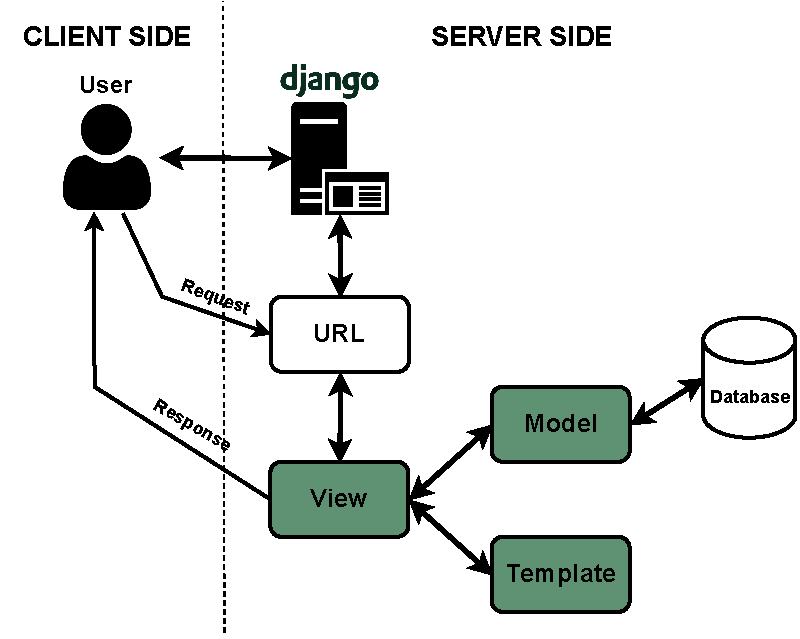
\includegraphics[width=0.7\textwidth]{figures/django_architecture.pdf}
    \caption{An architecture diagram showing the MVT design pattern of Django web applications.}
    \label{fig:django_architecture}
\end{figure}

Django has an intermediary component that catches the client's HTTP requests to pattern-match requested URLs to the correct view. The view then fetches data from the models stored in the backend, and renders a template back to the client.


\section{Backend Structure}
\subsection{Static Image Collection}
In line with requirement \textbf{\#\ref{req:18}}, several sources for image collections were considered. Out of those, there were two notable sources: the Wikimedia Commons and ImageNet. Wikimedia Commons hosts a range of images that are more importantly captioned with accurate textual descriptions. In addition to the latest multimodal, multilingual image-text dataset released by \cite{srinivasan2021wit}, a research group within Google. It appeared to be an appealing option as it allowed the flexibility to train our own image-text model using the provided textual descriptions. However, complications arose in downloading the dataset. We found that in order to save space, the dataset only included image URLs meaning that the images must be programmatically downloaded one by one. After weeks of testing, even going as far as parallelising the download process, we deemed this effort as infeasible due to its slow pace. 

We ultimately decided on procuring the collection from ImageNet, an open-source image database containing over 14 million images, available in zipped formats. Moreover, it provided many smaller subsets of the database that allowed the chance to familiarise ourselves with the CLIP's pre-training model architecture. The ImageNet-1k subset was the chosen collection for our project which spanned over 1 million images allowing reasonable pre-processing times while also being large enough for satisfactory image retrieval results.


\subsection{Models}
Our application consists of only two models: Audio and Chunks. As depicted in the Entity Relation (ER) diagram in Figure \ref{fig:models_schema}, each Audio object consists of 0 or more Chunk objects. This was to accommodate for purely instrumental audio tracks that would contain no spoken language. While this is not useful for our current application domain, we believed this feature could be expanded upon in future iterations where the audio content itself could be used in the image retrieval process using sentiment analysis.

\subsubsection{Audio}
The Audio model holds all information associated with inputted audio sources after processing is complete. This includes the artist/author's name, title, transcript, and the ground-truth data. A boolean flag for whether the audio is a music track or not is be used to course the appropriate processing steps. The file name field is be used to find corresponding files stored in the static directory, such as the audio, cover art image, or transcript files. 

\subsubsection{Chunk}
The Chunk model consists of specific information about the segment in the audio such as the text present, start and end times and finally, the top-10 and labelled images. It also holds a foreign key that references the appropriate Audio object.

\begin{figure}
    \centering
    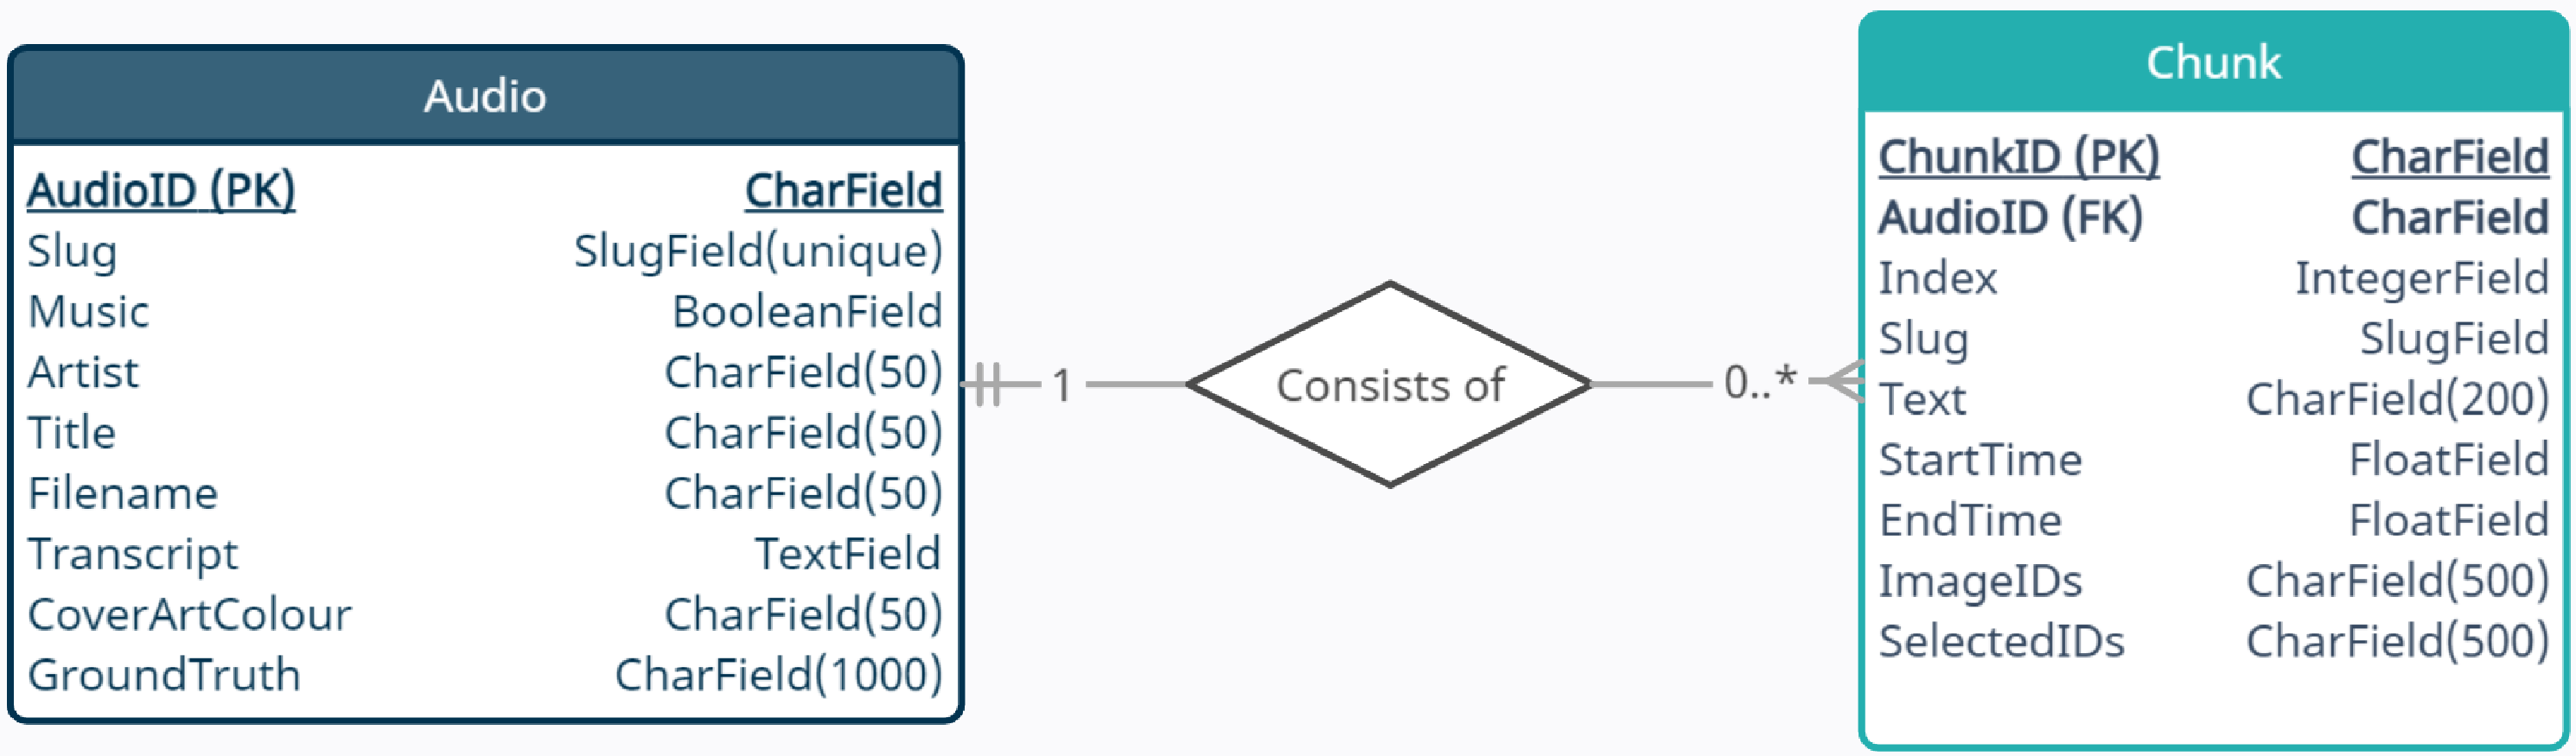
\includegraphics[width=1\textwidth]{figures/models_schema.pdf}
    \caption{An Entity Relation diagram showing the database schema made through Django models.}
    \label{fig:models_schema}
\end{figure}


\section{Program Structure}
All the main functionality is performed in the View component, represented by the file, \textbf{views.py}. However, each individual component outlined in the system architecture are abstracted into their own Python file in order to adhere to best software engineering practices. Each file, found in the \lstinline|utilities| folder, provides the required functions to accomplish a single task. This makes locating and adding functionality much easier comparative to an unorganised program structure.

\subsection{Audio Retriever}
Represented in the \textbf{audio\_retriever.py} file, this component lends functions that will be used to extract the audio file from the user's submission on the Home page. Firstly, the \textbf{\lstinline|home|} view will clear the \lstinline|audio| and \lstinline|transcript| directories in order to save space. Next, the client's HTTP POST request will be analysed to extract the YouTube video URL or uploaded audio file. In the case of the YouTube video URL, the \textbf{\lstinline|download_yt|} function is called in order to isolate and download the audio from the video using the library pytube \citep{pytube}. This function also retrieves the English or Automated English captions if present as well as saving the thumnail picture as the cover art, since these can be pulled from the resulting \textbf{\lstinline|pytube.Youtube|} object. Alternatively, in the case of a file upload, the file will be validated if it's of an audio format and then saved into the \lstinline|audio| folder for further processing.


\subsection{Audio Recogniser}
Now that the audio source is saved within the \lstinline|audio| folder, it can be processed in order to identify its track title and artist name assuming it is a music track. The \textbf{\lstinline|recognise_audio|} function attempts to match the audio source to a known music track using ShazamAPI \citep{shazamapi}. This API also provides the cover art URL for successful recognitions, meaning that this cover art is downloaded and saved within the \lstinline|coverart| folder using the HTTP Python library, Requests \citep{requests}. In addition to this, at later iterations it was decided to use the primary colour of the cover art to further visually differentiate audio sources (\textbf{\#\ref{req:31}}). For this the library ColorThief \citep{colorthief} to use image processing to identify the primary colour of the cover art which is then used to theme pages and links associated to the audio source.


\subsection{Synced Transcription Retriever}
This component holds multiple strategies to obtain a synced transcription of the audio in the LyRiCs (LRC) file format \citep{lrc}. The first method is retrieving the synced lyrics from the \cite{musixmatch} platform which holds an extensive database of song lyrics that are aligned with the song itself. The database is queried using the identified song title and artist name. If successsful, the lyrics are saved within the \lstinline|transcript| folder, as well as the external database within the Audio model. Evidently, this method only works with music tracks and so the component also provides the capability of robust audio-to-text transcription, leveraging OpenAI's Whisper model \citep{whisper}. Due to the memory limitations, only the \emph{'small'} model is loaded which was found to frequently misidentify words, hence its last resort status.  The resulting transcription is then formatted into the required LRC format.

This the last processing step within the \textbf{\lstinline|home|} view which will conclude by instantiating a new Audio object using the obtained information. For non-music, the title field is filled in with the YouTube video title or uploaded file name. While the artist field being the video creator or simply left as empty for uploaded files. Finally, the user is redirected to the Audio page.

The \textbf{\lstinline|audio|} view divides the transcript using the phrase-level timings and initialises new Chunk objects for each segment denoted by new lines in the rendered Audio page. Each new line is clickable link to the corresponding Chunk page. For audio sources with no spoken language, no transcription is made and instead the user is notified in the rendered Audio page.


\subsection{Image Retriever}
The \textbf{image\_retriever.py} file is responsible for image pre-processing and retrieval. In order to facilitate the freedom to configure the type of pre-trained CLIP model to use, a custom \textbf{\lstinline{CLIP}} class was made. This class holds properties such as the loaded model, tokenizer and processor, as well as the file paths for all images and their corresponding embedding vectors. We chose to use the CLIP ViT-B/32 model for its moderate size for reasonable loading times and its high performance. However, this model was trained with only English text and so to accommodate our requirement to support multiple languages (\textbf{\#\ref{req:12}}), we use a compatible Multilingual CLIP model that supports 100 languages, XLM-Roberta Large ViT-B/32 \citep{mclip}. Due to limited memory capacity, only one model can be loaded at one time so a Boolean flag is used to decide which model is loaded. Both models encode images and text into 512 dimensions of latent space and utilise the same vision transformer so can be interchanged according to the use case.

All images in the collection were pre-processed and embedded in batches using the pre-trained CLIP model and processor, to create a normalised NumPy matrix. This matrix was subsequently saved in a file so that it can be loaded into memory on application start-up. 

\label{sec:image_retriever:par:query_prompt}
The top 10 images are dynamically retrieved when a Chunk page is requested, handled by the \textbf{\lstinline{chunk}} view. The \textbf{\lstinline{query_prompt}} function takes in a text prompt, tokenizes it and embeds it into the 512-dimensional feature space using the pre-loaded model and tokenizer. Following this, an exhaustive similarity search is performed, this involves calculating the cosine similarity between the embedded text vector with every image vector stored in the matrix. Since all vectors are normalised beforehand by their Euclidean (L2) norm as demonstrated in Equation \ref{eq:euclidean_normalisation}, the cosine similarity score is simply the dot product between the vectors, accomplished with \textbf{\lstinline{numpy.dot(text_emb, image_embs.T)}}. 

$$\text{normalise}(\vec{x}) = \frac{\vec{x}}{\norm{\vec{x}}_2}$$

\begin{equation}
    \norm{\vec{x}}_2 = \sqrt{\sum_{i=1}^N \abs{x_i}^2} = \sqrt{x_1^2 + x_2^2 + ... + x_N^2}
    \label{eq:euclidean_normalisation}
\end{equation}

These similarity scores are subsequently sorted in descending order to get the 10 images that scored the highest with the text query which is then listed to the user on the Chunk page. In order to save unnecessary computation, these image indices are saved in the database associated to the Chunk object.


\subsection{Ground-Truth Builder}
Following the wireframes laid out during the design, the annotator can click on the 'Build Ground Truth' button on the Audio page and is thereafter transported to the first Chunk page to begin the relevance assessment task. As explained in \ref{sec:image_retriever:par:query_prompt}, the \textbf{\lstinline|query_prompt|} function will be called on a ad-hoc basis for each chunk in order to display the highest scoring images. The annotator can then label the most fitting images by placing a check mark to denote relevance. This application uses the jQuery plugin, imgCheckbox \citep{imgcheckbox}, to dynamically inject checkboxes onto HTML \textbf{\lstinline|<img>|} tags on the webpage. 

All annotated images are saved within the Chunk object when the user submits a HTTP POST request which can occur when the 'Previous' or 'Next' buttons are pressed. This allows previously annotated Chunks to be viewed and amended fulfilling requirement \textbf{\#\ref{req:11}}. Additionally, throughout testing it was found to be burdensome to annotate chunks with repeating textual content, leading to the addition of requirement \textbf{\#\ref{req:16}}. This feature greatly reduced annotation effort and efficiency since all duplicate chunks can be updated at once and skipped during relevance assessment.

The full ground truth can only be viewed when the user clicks the 'Finish' button on the last chunk of the transcript. The ground truth is built chunk by chunk, appending to a Python dictionary storing relevant information of the audio source and chunks. The indices of the assessed images are stored here as well as their corresponding file paths in order to ease evaluation. In order to release the data in a human-readable and easily accessible format (\textbf{\#\ref{req:9}}), the resulting Python dictionary is serialised into JavaScript Object Notation (JSON) \citep{json}. This format is an open standard format that is language-independant. A preview of the data is subsequently rendered in the Ground-Truth page with a clear button to download it.

\subsubsection{Determining Pooling Depth}
The final pooling depth of $k=10$ was determined through trial and error, since it was difficult to estimate the effectiveness of CLIP models on multi-conceptual text prompts that is so common in spoken language and especially song lyrics. Retrieving the top-10 images was determined to be the ideal depth that is able to be fit in one page without excessive rescaling as well as not increasing relevance assessment effort. However, it was noticed that in rare occasions of extreme ambiguity of text, more images were required to be assessed to find any relevance. This was also picked up during user evaluations in (REF) where it may be beneficial to increase $k$ for very abstract ideas.


\subsection{Video Compiler}
The video compiler component implemented in the \textbf{videography.py} file, takes care of generating the video primarily using the library MoviePy \citep{moviepy}. The video is built incrementally, much like the ground-truth construction, by selecting the top-1 image for each chunk and concatenating \textbf{\lstinline|ImageClip|s} in sequence, with their durations being the difference between the chunk start and end timestamps. \textbf{\lstinline|TextClip|s} showing the chunk text are placed below corresponding images. Parts of the audio lacking spoken words are filled with blank \textbf{\lstinline|ColorClip|s}. Lastly, the audio source is added to the final \textbf{\lstinline|VideoClip|} which is then written into an MP4 file in the \lstinline|video| folder. This file is then embedded into the HTML of the Video page for the user to play and download the generated video.


% \subsection{Templates}
\section{Summary}
This chapter described the steps taken in manifesting the blueprint designs into a concrete product. Key implementation details were explained as well as the challenges faced along the process. Rationale for the chosen language and web framework were given, in addition to how the various libraries were integrated into the project in order to reduce the complexity of the project's development. A full account of the program's structure and technical accomplishments were given. Now that the application has been fully implemented, it presents an opportunity to assess its efficacy in achieving the project's intended goals.

% What did you do to implement this idea, and what technical achievements did you make?
% \section{Guidance}
% You can't talk about everything. Cover the high level first, then cover important, relevant or impressive details.

% \section{General guidance for technical writing}

% These points apply to the whole dissertation, not just this chapter.

% \subsection{Figures}
% \emph{Always} refer to figures included, like Figure \ref{fig:relu}, in the body of the text. Include full, explanatory captions and make sure the figures look good on the page.
% You may include multiple figures in one float, as in Figure \ref{fig:synthetic}, using \texttt{subcaption}, which is enabled in the template.


% % Figures are important. Use them well.
% \begin{figure}[htb]
%     \centering
%     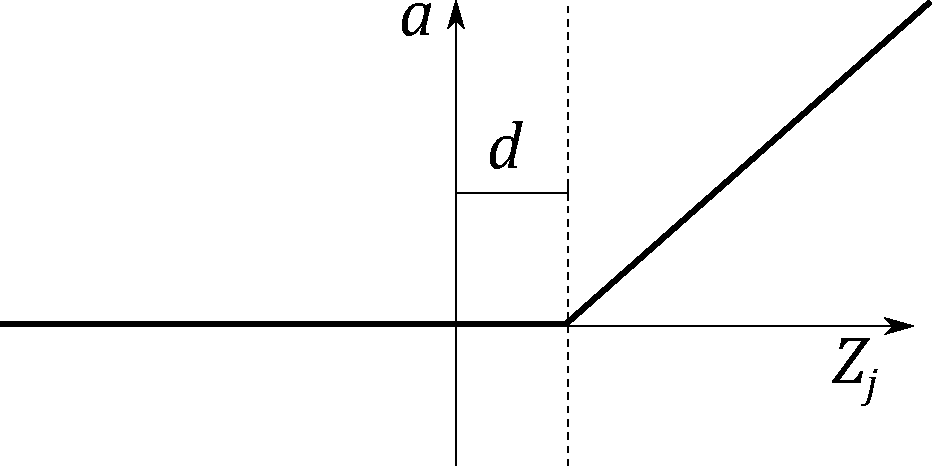
\includegraphics[width=0.5\linewidth]{figures/relu.pdf}    

%     \caption{In figure captions, explain what the reader is looking at: ``A schematic of the rectifying linear unit, where $a$ is the output amplitude,
%     $d$ is a configurable dead-zone, and $Z_j$ is the input signal'', as well as why the reader is looking at this: 
%     ``It is notable that there is no activation \emph{at all} below 0, which explains our initial results.'' 
%     \textbf{Use vector image formats (.pdf) where possible}. Size figures appropriately, and do not make them over-large or too small to read.
%     }

%     % use the notation fig:name to cross reference a figure
%     \label{fig:relu} 
% \end{figure}


% \begin{figure}[htb] 
%     \centering
%     \begin{subfigure}[b]{0.45\textwidth}
%         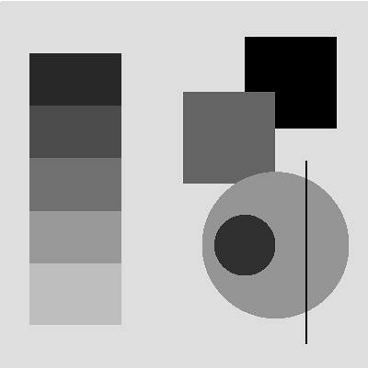
\includegraphics[width=\textwidth]{figures/synthetic.png}
%         \caption{Synthetic image, black on white.}
%         \label{fig:syn1}
%     \end{subfigure}
%     ~ %add desired spacing between images, e. g. ~, \quad, \qquad, \hfill etc. 
%       %(or a blank line to force the subfigure onto a new line)
%     \begin{subfigure}[b]{0.45\textwidth}
%         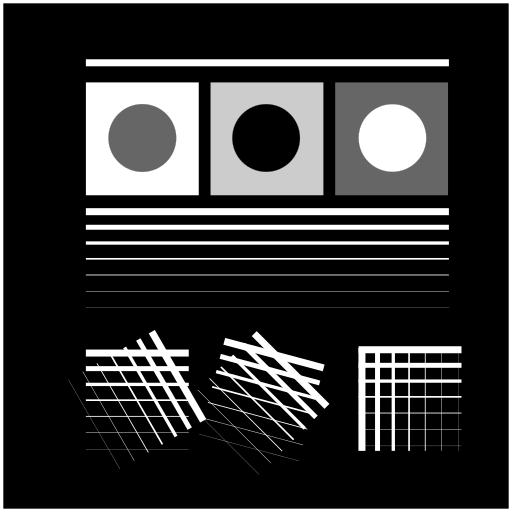
\includegraphics[width=\textwidth]{figures/synthetic_2.png}
%         \caption{Synthetic image, white on black.}
%         \label{fig:syn2}
%     \end{subfigure}
%     ~ %add desired spacing between images, e. g. ~, \quad, \qquad, \hfill etc. 
%     %(or a blank line to force the subfigure onto a new line)    
%     \caption{Synthetic test images for edge detection algorithms. \subref{fig:syn1} shows various gray levels that require an adaptive algorithm. \subref{fig:syn2}
%     shows more challenging edge detection tests that have crossing lines. Fusing these into full segments typically requires algorithms like the Hough transform.
%     This is an example of using subfigures, with \texttt{subref}s in the caption.
%     }\label{fig:synthetic}
% \end{figure}

% \clearpage

% \subsection{Equations}

% Equations should be typeset correctly and precisely. Make sure you get parenthesis sizing correct, and punctuate equations correctly 
% (the comma is important and goes \textit{inside} the equation block). Explain any symbols used clearly if not defined earlier. 

% For example, we might define:
% \begin{equation}
%     \hat{f}(\xi) = \frac{1}{2}\left[ \int_{-\infty}^{\infty} f(x) e^{2\pi i x \xi} \right],
% \end{equation}    
% where $\hat{f}(\xi)$ is the Fourier transform of the time domain signal $f(x)$.

% \subsection{Algorithms}
% Algorithms can be set using \texttt{algorithm2e}, as in Algorithm \ref{alg:metropolis}.

% % NOTE: line ends are denoted by \; in algorithm2e
% \begin{algorithm}
%     \DontPrintSemicolon
%     \KwData{$f_X(x)$, a probability density function returing the density at $x$.\; $\sigma$ a standard deviation specifying the spread of the proposal distribution.\;
%     $x_0$, an initial starting condition.}
%     \KwResult{$s=[x_1, x_2, \dots, x_n]$, $n$ samples approximately drawn from a distribution with PDF $f_X(x)$.}
%     \Begin{
%         $s \longleftarrow []$\;
%         $p \longleftarrow f_X(x)$\;
%         $i \longleftarrow 0$\;
%         \While{$i < n$}
%         {
%             $x^\prime \longleftarrow \mathcal{N}(x, \sigma^2)$\;
%             $p^\prime \longleftarrow f_X(x^\prime)$\;
%             $a \longleftarrow \frac{p^\prime}{p}$\;
%             $r \longleftarrow U(0,1)$\;
%             \If{$r<a$}
%             {
%                 $x \longleftarrow x^\prime$\;
%                 $p \longleftarrow f_X(x)$\;
%                 $i \longleftarrow i+1$\;
%                 append $x$ to $s$\;
%             }
%         }
%     }
    
% \caption{The Metropolis-Hastings MCMC algorithm for drawing samples from arbitrary probability distributions, 
% specialised for normal proposal distributions $q(x^\prime|x) = \mathcal{N}(x, \sigma^2)$. The symmetry of the normal distribution means the acceptance rule takes the simplified form.}\label{alg:metropolis}
% \end{algorithm}

% \subsection{Tables}

% If you need to include tables, like Table \ref{tab:operators}, use a tool like https://www.tablesgenerator.com/ to generate the table as it is
% extremely tedious otherwise. 

% \begin{table}[]
%     \caption{The standard table of operators in Python, along with their functional equivalents from the \texttt{operator} package. Note that table
%     captions go above the table, not below. Do not add additional rules/lines to tables. }\label{tab:operators}
%     %\tt 
%     \rowcolors{2}{}{gray!3}
%     \begin{tabular}{@{}lll@{}}
%     %\toprule
%     \textbf{Operation}    & \textbf{Syntax}                & \textbf{Function}                            \\ %\midrule % optional rule for header
%     Addition              & \texttt{a + b}                          & \texttt{add(a, b)}                                    \\
%     Concatenation         & \texttt{seq1 + seq2}                    & \texttt{concat(seq1, seq2)}                           \\
%     Containment Test      & \texttt{obj in seq}                     & \texttt{contains(seq, obj)}                           \\
%     Division              & \texttt{a / b}                          & \texttt{div(a, b) }  \\
%     Division              & \texttt{a / b}                          & \texttt{truediv(a, b) } \\
%     Division              & \texttt{a // b}                         & \texttt{floordiv(a, b)}                               \\
%     Bitwise And           & \texttt{a \& b}                         & \texttt{and\_(a, b)}                                  \\
%     Bitwise Exclusive Or  & \texttt{a \textasciicircum b}           & \texttt{xor(a, b)}                                    \\
%     Bitwise Inversion     & \texttt{$\sim$a}                        & \texttt{invert(a)}                                    \\
%     Bitwise Or            & \texttt{a | b}                          & \texttt{or\_(a, b)}                                   \\
%     Exponentiation        & \texttt{a ** b}                         & \texttt{pow(a, b)}                                    \\
%     Identity              & \texttt{a is b}                         & \texttt{is\_(a, b)}                                   \\
%     Identity              & \texttt{a is not b}                     & \texttt{is\_not(a, b)}                                \\
%     Indexed Assignment    & \texttt{obj{[}k{]} = v}                 & \texttt{setitem(obj, k, v)}                           \\
%     Indexed Deletion      & \texttt{del obj{[}k{]}}                 & \texttt{delitem(obj, k)}                              \\
%     Indexing              & \texttt{obj{[}k{]}}                     & \texttt{getitem(obj, k)}                              \\
%     Left Shift            & \texttt{a \textless{}\textless b}       & \texttt{lshift(a, b)}                                 \\
%     Modulo                & \texttt{a \% b}                         & \texttt{mod(a, b)}                                    \\
%     Multiplication        & \texttt{a * b}                          & \texttt{mul(a, b)}                                    \\
%     Negation (Arithmetic) & \texttt{- a}                            & \texttt{neg(a)}                                       \\
%     Negation (Logical)    & \texttt{not a}                          & \texttt{not\_(a)}                                     \\
%     Positive              & \texttt{+ a}                            & \texttt{pos(a)}                                       \\
%     Right Shift           & \texttt{a \textgreater{}\textgreater b} & \texttt{rshift(a, b)}                                 \\
%     Sequence Repetition   & \texttt{seq * i}                        & \texttt{repeat(seq, i)}                               \\
%     Slice Assignment      & \texttt{seq{[}i:j{]} = values}          & \texttt{setitem(seq, slice(i, j), values)}            \\
%     Slice Deletion        & \texttt{del seq{[}i:j{]}}               & \texttt{delitem(seq, slice(i, j))}                    \\
%     Slicing               & \texttt{seq{[}i:j{]}}                   & \texttt{getitem(seq, slice(i, j))}                    \\
%     String Formatting     & \texttt{s \% obj}                       & \texttt{mod(s, obj)}                                  \\
%     Subtraction           & \texttt{a - b}                          & \texttt{sub(a, b)}                                    \\
%     Truth Test            & \texttt{obj}                            & \texttt{truth(obj)}                                   \\
%     Ordering              & \texttt{a \textless b}                  & \texttt{lt(a, b)}                                     \\
%     Ordering              & \texttt{a \textless{}= b}               & \texttt{le(a, b)}                                     \\
%     % \bottomrule
%     \end{tabular}
%     \end{table}
% \subsection{Code}

% Avoid putting large blocks of code in the report (more than a page in one block, for example). Use syntax highlighting if possible, as in Listing \ref{lst:callahan}.

% \begin{lstlisting}[language=python, float, caption={The algorithm for packing the $3\times 3$ outer-totalistic binary CA successor rule into a 
%     $16\times 16\times 16\times 16$ 4 bit lookup table, running an equivalent, notionally 16-state $2\times 2$ CA.}, label=lst:callahan]
%     def create_callahan_table(rule="b3s23"):
%         """Generate the lookup table for the cells."""        
%         s_table = np.zeros((16, 16, 16, 16), dtype=np.uint8)
%         birth, survive = parse_rule(rule)

%         # generate all 16 bit strings
%         for iv in range(65536):
%             bv = [(iv >> z) & 1 for z in range(16)]
%             a, b, c, d, e, f, g, h, i, j, k, l, m, n, o, p = bv

%             # compute next state of the inner 2x2
%             nw = apply_rule(f, a, b, c, e, g, i, j, k)
%             ne = apply_rule(g, b, c, d, f, h, j, k, l)
%             sw = apply_rule(j, e, f, g, i, k, m, n, o)
%             se = apply_rule(k, f, g, h, j, l, n, o, p)

%             # compute the index of this 4x4
%             nw_code = a | (b << 1) | (e << 2) | (f << 3)
%             ne_code = c | (d << 1) | (g << 2) | (h << 3)
%             sw_code = i | (j << 1) | (m << 2) | (n << 3)
%             se_code = k | (l << 1) | (o << 2) | (p << 3)

%             # compute the state for the 2x2
%             next_code = nw | (ne << 1) | (sw << 2) | (se << 3)

%             # get the 4x4 index, and write into the table
%             s_table[nw_code, ne_code, sw_code, se_code] = next_code

%         return s_table

% \end{lstlisting}

%==================================================================================================
\chapter{Evaluation} 
(FAISS)

(VIDEO GENERATION RUNTIME EXPERIMENTS)

(SHOULD ASSESSORS PICK CLEAR IMAGES)

\begin{figure}
    \centering
    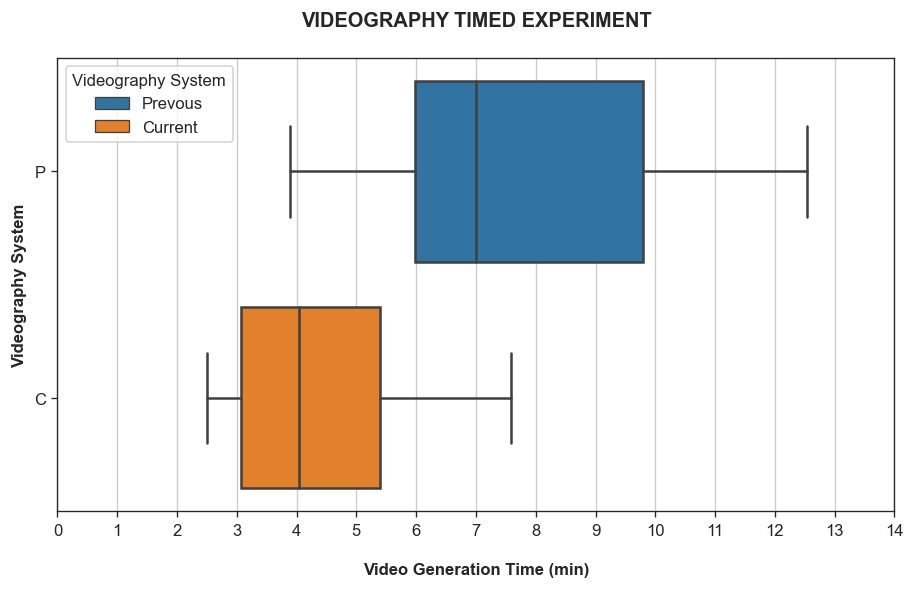
\includegraphics[width=1\textwidth]{figures/videography_timed_experiment.png}
    \caption{describe}
    \label{fig:videography_timed}
\end{figure}

% How good is your solution? How well did you solve the general problem, and what evidence do you have to support that?

% \section{Guidance}
% \begin{itemize}
%     \item
%         Ask specific questions that address the general problem.
%     \item
%         Answer them with precise evidence (graphs, numbers, statistical
%         analysis, qualitative analysis).
%     \item
%         Be fair and be scientific.
%     \item
%         The key thing is to show that you know how to evaluate your work, not
%         that your work is the most amazing product ever.
% \end{itemize}

% \section{Evidence}
% Make sure you present your evidence well. Use appropriate visualisations, 
% reporting techniques and statistical analysis, as appropriate. The point is not
% to dump all the data you have but to present an argument well supported by evidence gathered.

% If you use numerical evidence, specify reasonable numbers of significant digits; don't state ``18.41141\% of users were successful'' if you only had 20 users. If you average \textit{anything}, present both a measure of central tendency (e.g. mean, median) \textit{and} a measure of spread (e.g. standard deviation, min/max, interquartile range).

% You can use \texttt{siunitx} to define units, space numbers neatly, and set the precision for the whole LaTeX document. 

% % setup siunitx to have two decimal places
% \sisetup{
% 	round-mode = places,
% 	round-precision = 2
% }

% For example, these numbers will appear with two decimal places: \num{3.141592}, \num{2.71828}, and this one will appear with reasonable spacing \num{1000000}.



% If you use statistical procedures, make sure you understand the process you are using,
% and that you check the required assumptions hold in your case. 

% If you visualise, follow the basic rules, as illustrated in Figure \ref{fig:boxplot}:
% \begin{itemize}
% \item Label everything correctly (axis, title, units).
% \item Caption thoroughly.
% \item Reference in text.
% \item \textbf{Include appropriate display of uncertainty (e.g. error bars, Box plot)}
% \item Minimize clutter.
% \end{itemize}

% See the file \texttt{guide\_to\_visualising.pdf} for further information and guidance.

% \begin{figure}[htb]
%     \centering
%     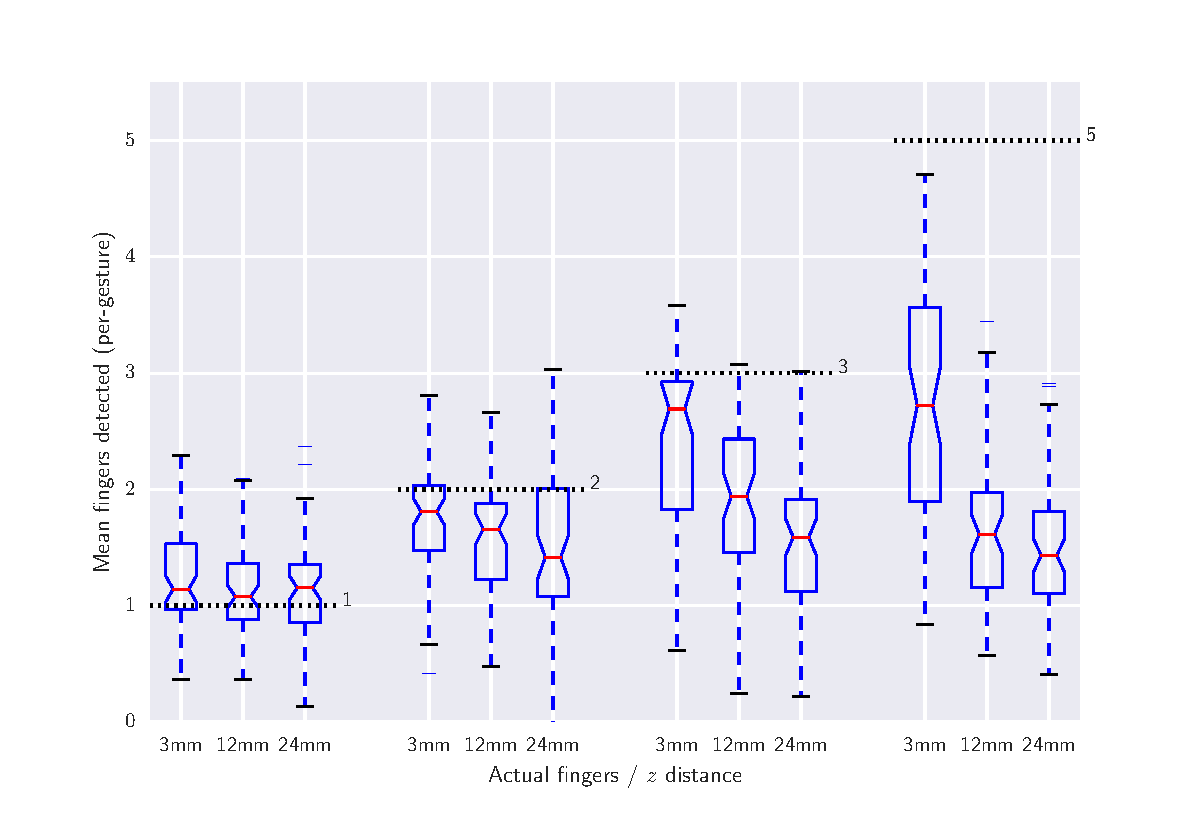
\includegraphics[width=1.0\linewidth]{figures/boxplot_finger_distance.pdf}    

%     \caption{Average number of fingers detected by the touch sensor at different heights above the surface, averaged over all gestures. Dashed lines indicate
%     the true number of fingers present. The Box plots include bootstrapped uncertainty notches for the median. It is clear that the device is biased toward 
%     undercounting fingers, particularly at higher $z$ distances.
%     }

%     % use the notation fig:name to cross reference a figure
%     \label{fig:boxplot} 
% \end{figure}


%==================================================================================================
\chapter{Conclusion}    
Summarise the whole project for a lazy reader who didn't read the rest (e.g. a prize-awarding committee). This chapter should be short in most dissertations; maybe one to three pages.
\section{Guidance}
\begin{itemize}
    \item
        Summarise briefly and fairly.
    \item
        You should be addressing the general problem you introduced in the
        Introduction.        
    \item
        Include summary of concrete results (``the new compiler ran 2x
        faster'')
    \item
        Indicate what future work could be done, but remember: \textbf{you
        won't get credit for things you haven't done}.
\end{itemize}

\section{Summary}
Summarise what you did; answer the general questions you asked in the introduction. What did you achieve? Briefly describe what was built and summarise the evaluation results.

\section{Reflection}
Discuss what went well and what didn't and how you would do things differently if you did this project again.

\section{Future work}
Discuss what you would do if you could take this further -- where would the interesting directions to go next be? (e.g. you got another year to work on it, or you started a company to work on this, or you pursued a PhD on this topic)

%==================================================================================================
%  APPENDICES  

\begin{appendices}

\chapter{Appendices}
 (ETHICS CHECKLIST + INTRODUCTION BRIEF)
 
Use separate appendix chapters for groups of ancillary material that support your dissertation. 
Typical inclusions in the appendices are:

\begin{itemize}
\item
  Copies of ethics approvals (you must include these if you needed to get them)
\item
  Copies of questionnaires etc. used to gather data from subjects. Don't include
  voluminous data logs; instead submit these electronically alongside your source code.
\item
  Extensive tables or figures that are too bulky to fit in the main body of
  the report, particularly ones that are repetitive and summarised in the body.
\item Outline of the source code (e.g. directory structure), 
    or other architecture documentation like class diagrams.
\item User manuals, and any guides to starting/running the software. 
Your equivalent of \texttt{readme.md} should be included.

\end{itemize}

\textbf{Don't include your source code in the appendices}. It will be
submitted separately.

\chapter{Video Generation Experiment}
\begin{table}
    \centering
    % \rowcolors{2}{}{gray!3}
    \begin{tabular}{|c|c|c|}
        \hline
        \textbf{Audio Source} & \textbf{Runtime \lstinline|(mm:ss)|} & \textbf{Number of Chunks} \\
        \hline
        \hline
        1 & 04:37 & 61 \\
        \hline
        2 & 02:25 & 42 \\
        \hline
        3 & 02:26 & 62 \\
        \hline
        4 & 03:58 & 81 \\
        \hline
        5 & 04:34 & 80 \\
        \hline
        6 & 04:30 & 62 \\
        \hline
        7 & 02:03 & 34 \\
        \hline
        8 & 03:10 & 36 \\
        \hline
        9 & 04:23 & 53 \\
        \hline
        10 & 03:26 & 69 \\
        \hline
        11 & 04:05 & 74 \\
        \hline
        12 & 03:08 & 51 \\
        \hline
        13 & 04:38 & 36 \\
        \hline
        14 & 04:04 & 21 \\
        \hline
        15 & 03:49 & 37 \\
        \hline
        16 & 03:20 & 38 \\
        \hline
        17 & 02:10 & 26 \\
        \hline
        18 & 04:09 & 43 \\
        \hline
        19 & 03:49 & 26 \\
        \hline
        20 & 04:40 & 26 \\
        \hline
    \end{tabular}
    \caption{The standard table of operators in Python, along with their functional equivalents from the \texttt{operator} package. Note that table
    captions go above the table, not below. Do not add additional rules/lines to tables. }\label{tab:audio_sources}
\end{table}

\begin{table}
    \centering
    \begin{tabular}{|c|c|c|}
        \hline
        \multirow{2}{*}{\textbf{Audio Source}} & 
        \multicolumn{2}{|c|}{\textbf{Video Generation Time \lstinline|(mm:ss)|}} \\
        \cline{2-3} & \textbf{Previous System} & \textbf{Current System} \\ 
        \hline
        \hline
        1 & 08:47 & 04:55 \\
        \hline
        2 & 06:55 & 02:30 \\
        \hline
        3 & 09:48 & 03:02 \\
        \hline
        4 & 12:32 & 07:10 \\
        \hline
        5 & 12:24 & 07:36 \\
        \hline
        6 & 09:48 & 06:09 \\
        \hline
        7 & 05:46 & 03:05 \\
        \hline
        8 & 06:03 & 04:43 \\
        \hline
        9 & 08:30 & 06:58 \\
        \hline
        10 & 10:49 & 05:08 \\
        \hline
        11 & 11:32 & 07:12 \\
        \hline
        12 & 08:13 & 04:16 \\
        \hline
        13 & 06:03 & 03:60 \\
        \hline
        14 & 03:54 & 02:48 \\
        \hline
        15 & 06:12 & 02:44 \\
        \hline
        16 & 06:21 & 03:35 \\
        \hline
        17 & 04:37 & 02:33 \\
        \hline
        18 & 07:04 & 04:04 \\
        \hline
        19 & 04:37 & 03:49 \\
        \hline
        20 & 04:37 & 03:15 \\
        \hline
    \end{tabular}
    \caption{The standard table of operators in Python, along with their functional equivalents from the \texttt{operator} package. Note that table
    captions go above the table, not below. Do not add additional rules/lines to tables. }\label{tab:videography_times}
\end{table}
\end{appendices}

%==================================================================================================
%   BIBLIOGRAPHY   

% The bibliography style is agsm (Harvard)
% The bibliography always appears last, after the appendices.

\bibliographystyle{agsm}

% Force the bibliography not to be numbered
\renewcommand{\thechapter}{0} 
\bibliography{l4proj}

\end{document}
